% !TeX encoding = utf8
\documentclass[aspectratio=169]{beamer}

\usepackage[ngerman]{babel}
\usepackage{amsmath}
\usepackage{amssymb}
\usepackage{quoting}
\usepackage{enumitem}
%\usepackage{mathpazo}
%\usepackage{palatino}
%\usefonttheme{professionalfonts}
\usepackage{libertine}
\usepackage[libertine]{newtxmath}
%\renewcommand\familydefault{\rmdefault}
%\usefonttheme[onlymath]{serif}

\definecolor{aica-green}{RGB}{214,255,237}
\definecolor{fg-aica}{RGB}{141,88,255}
\definecolor{bg-aica}{RGB}{28,28,28}
\definecolor{mygreen}{RGB}{85,168,104}
\definecolor{myred}{RGB}{196,78,82}


\setbeamercolor{structure}{bg=bg-aica,fg=fg-aica}
\setbeamercolor{title}{fg=white}
\setbeamercolor{frametitle}{fg=white}
\setbeamercolor{block title}{fg=white}
\setbeamercolor{definition}{fg=white}
\setbeamercolor{block body}{bg=aica-green}
\setbeamertemplate{navigation symbols}[only frame symbol]

\DeclareMathOperator*{\E}{\mathbf{E}}
\DeclareMathOperator*{\Prob}{\mathbf{P}}
\newcommand{\A}{\mathbf{A}}
\newcommand{\Pro}{\mathbf{P}}
\newcommand{\xx}{\mathbf{x}}
\newcommand{\bb}{\mathbf{b}}
\newcommand{\ee}{\mathbf{e}}
\newcommand{\pp}{\mathbf{p}}
\newcommand\inner[2]{\langle #1, #2 \rangle }
\newcommand{\R}{\mathbb{R}}

\DeclareMathOperator*{\argmax}{arg\,max}
\DeclareMathOperator*{\argmin}{arg\,min}

\addtobeamertemplate{navigation symbols}{}{%
	\usebeamerfont{footline}%
	\usebeamercolor[fg]{footline}%
	\hspace{1em}%
	\insertframenumber/\inserttotalframenumber
}

\AtBeginSection[]{
	\begin{frame}
		\vfill
		\centering
		\begin{beamercolorbox}[sep=8pt,center,shadow=true,rounded=true]{title}
			\usebeamerfont{title}\insertsectionhead\par%
		\end{beamercolorbox}
		\vfill
	\end{frame}
}

\title{Algorithmische Komposition mit Neuronalen Netzen}
\subtitle{AICA Crashkurs}
\author{\href{mailto:zoennchen.benedikt@hm.edu}{\textbf{Benedikt Z\"onnchen}}} 
\date{\today}
%\setdefaultlanguage[spelling=new]{german}
\graphicspath{{./../figs/}}

\begin{document}
	
\begin{frame}
	\titlepage
\end{frame}

\begin{frame}
	\frametitle{Inhalt}
	\tableofcontents
\end{frame}

\begin{frame}
	\begin{columns}
		\begin{column}{0.7\textwidth}
				\begin{quoting}
				``[The mechanical engine] might act upon other things besides numbers, were objects found whose mutual fundamental relations could be expressed by those of the abstract science of operations, and which should be also susceptible of adaptations to the action of the operating notation and mechanism of the engine. […] Supposing, for instance, that the fundamental relations of pitched sounds in the science of harmony and of musical composition were susceptible of such expression and adaptations, the engine might compose elaborate and scientific pieces of music of any degree of complexity or extent.'' -- Ada Lovelace (1815 - 1852)
			\end{quoting}
		\end{column}
		\begin{column}{0.3\textwidth}
			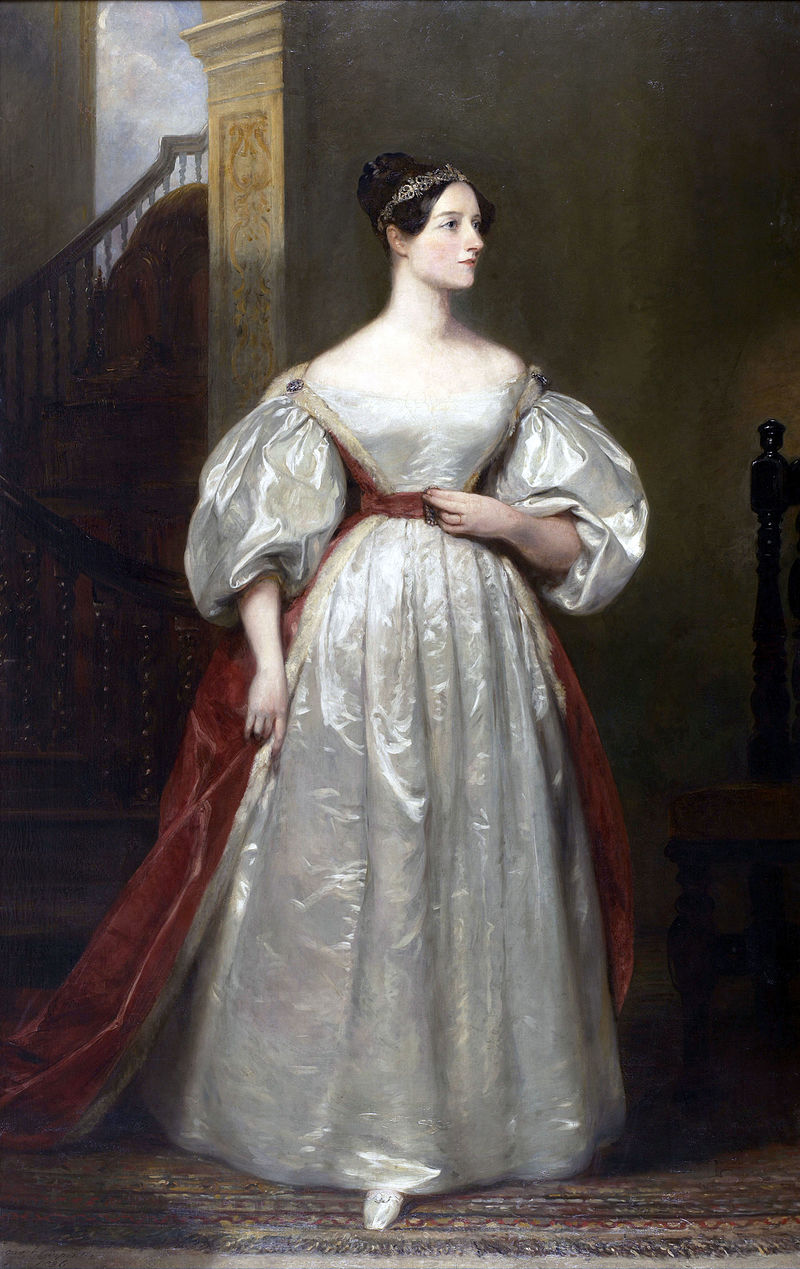
\includegraphics[width=\textwidth]{ada}
		\end{column}
	\end{columns}
\end{frame}

\section{Einleitung}

\begin{frame}
	\frametitle{Einleitung: Problemdefinition}
	\begin{block}{Problem}
		Gegeben sei eine Sequenz von Noten der Länge $n \geq 0$. Generiere eine ``wohlklingende'' Fortsetzung.
	\end{block}
	\begin{figure}
		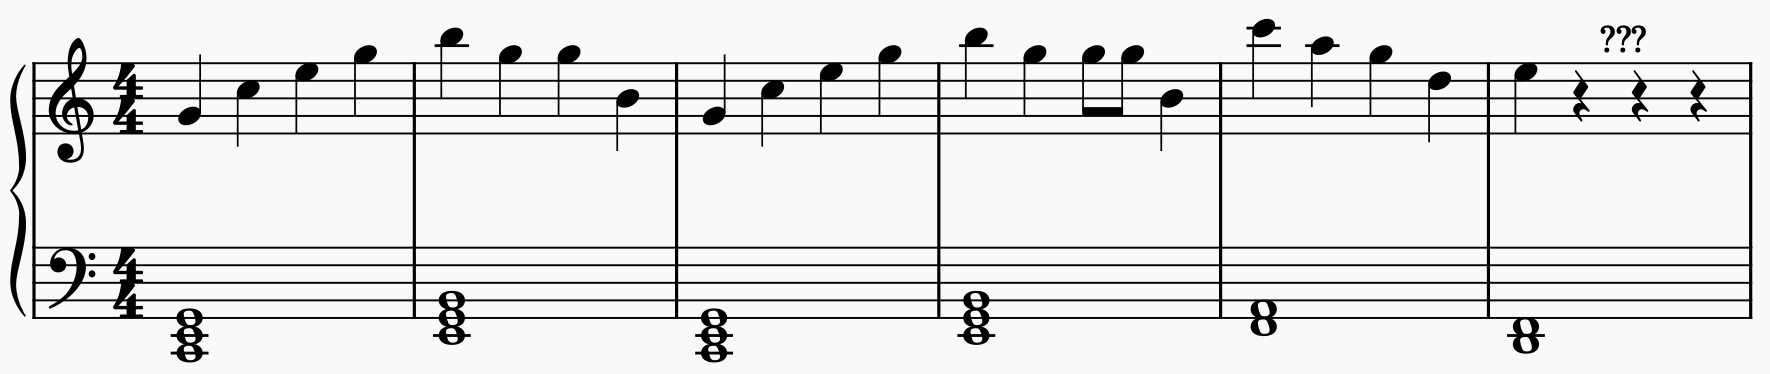
\includegraphics[width=\textwidth]{notes}
	\end{figure}
\end{frame}


\begin{frame}
	\frametitle{Einleitung}
	Die Generierung guter Melodien und Harmonien ist ein schwieriges Problem:
	\begin{enumerate}[label=$\bullet$]
		\item Mehrdimensionale Beziehungen (vertikale Harmonie und horizontale Melodie)
		\item Relative Beziehungen (Intervalle)
		\item Hoch-  und niederfrequente Beziehungen
		\item Teils einzigartige Stücke
		\item Spannung zwischen Wiederholung und Überraschung
		\item $\ldots$
	\end{enumerate}
	Anders als Sprache ist Musik ein Spiel mit Erwartungen -- ein Zusammenspiel aus Wiederholung und Überraschung.
\end{frame}

\begin{frame}
	\frametitle{Einleitung}
	\framesubtitle{Repräsentationen}
	%	\begin{quoting}
		%		``Music is the universal language of mankind.'' -- H. W. Longfellow
		%	\end{quoting}
	Die Beziehung zwischen symbolischer Notation und Ton ist ähnlich zur Beziehung zwischen Text und Sprache:
	\begin{enumerate}[label=$\bullet$]
		\item \textbf{Partitur}: Symbolisch, abstrakt, transportiert musikalische Gedanken
		\item \textbf{Ton}: Durchgängig, konkret, enthält alle Details
	\end{enumerate}
	
	Zwischen diesen beiden Extremen liegen oftmals weitere Schritte von abstrakt zu konkret.
\end{frame}

\begin{frame}
	\frametitle{Einleitung}
	\framesubtitle{Repräsentationen}
	\begin{figure}
		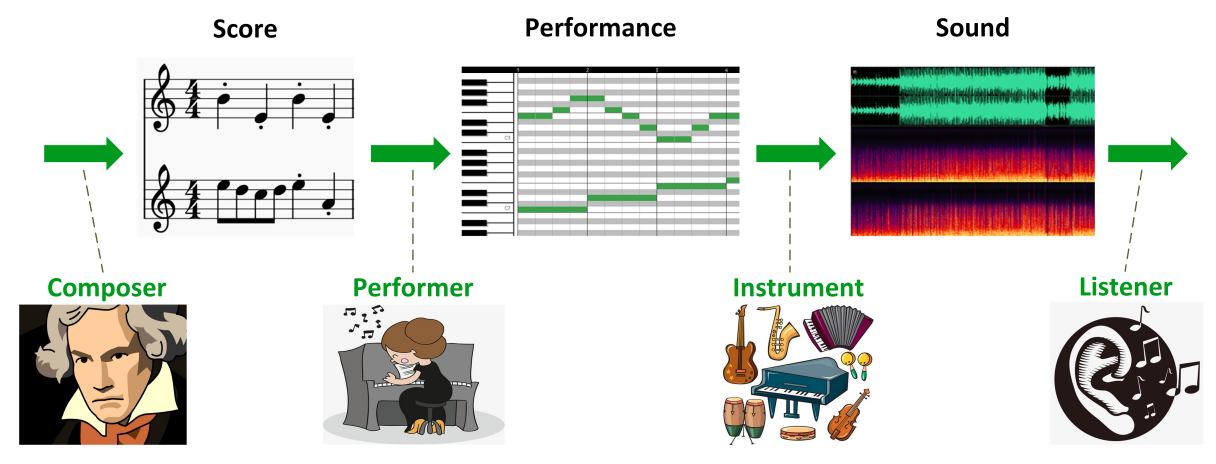
\includegraphics[width=\textwidth]{overview}
		\caption{Quelle: \cite{shulei:2020}}
	\end{figure}
\end{frame}

\begin{frame}
	\frametitle{Einleitung}
	\framesubtitle{Extreme der algorithmischen Komposition}
	Nach \cite{nierhaus:2010} können wir zwischen den Extremen
	\begin{enumerate}[label=$\bullet$]
		\item \textbf{authentische Komposition} und
		\item \textbf{Imitation} (des Stils),
	\end{enumerate}
	unterscheiden, wobei wir uns immer zwischen den Extremen befinden werden.
\end{frame}

\begin{frame}
	\frametitle{Einleitung}
	\framesubtitle{Extreme der algorithmischen Komposition}
	Zusätzlich können wir zwischen weiteren Extremen unterscheiden, nämlich
	\begin{enumerate}[label=$\bullet$]
		\item \textbf{regelbasierte} und 
		\item \textbf{datengetriebene},
	\end{enumerate}
	sowie
	\begin{enumerate}[label=$\bullet$]
		\item \textbf{automatisierte} und 
		\item \textbf{manuelle} Komposition.
	\end{enumerate}
\end{frame}

\begin{frame}
\frametitle{Einleitung}
\framesubtitle{Regelbasierte Techniken}
\begin{columns}
	\begin{column}{0.5\textwidth}
		\begin{block}{Regelbasierte Techniken}
		\begin{enumerate}[label=$\bullet$]
			\item \textbf{Markov-Chain (MC)}
			\item Hidden Markov Model (HMM)
			\item Zelluläre Automaten
			\item Generierende Grammatiken
			\item Lindenmayer-Systeme
			\item Fraktale
			\item Genetische Algorithmen
			\item $\ldots$
		\end{enumerate}
	\end{block}
	\end{column}
	
	\begin{column}{0.5\textwidth}
		\begin{figure}
			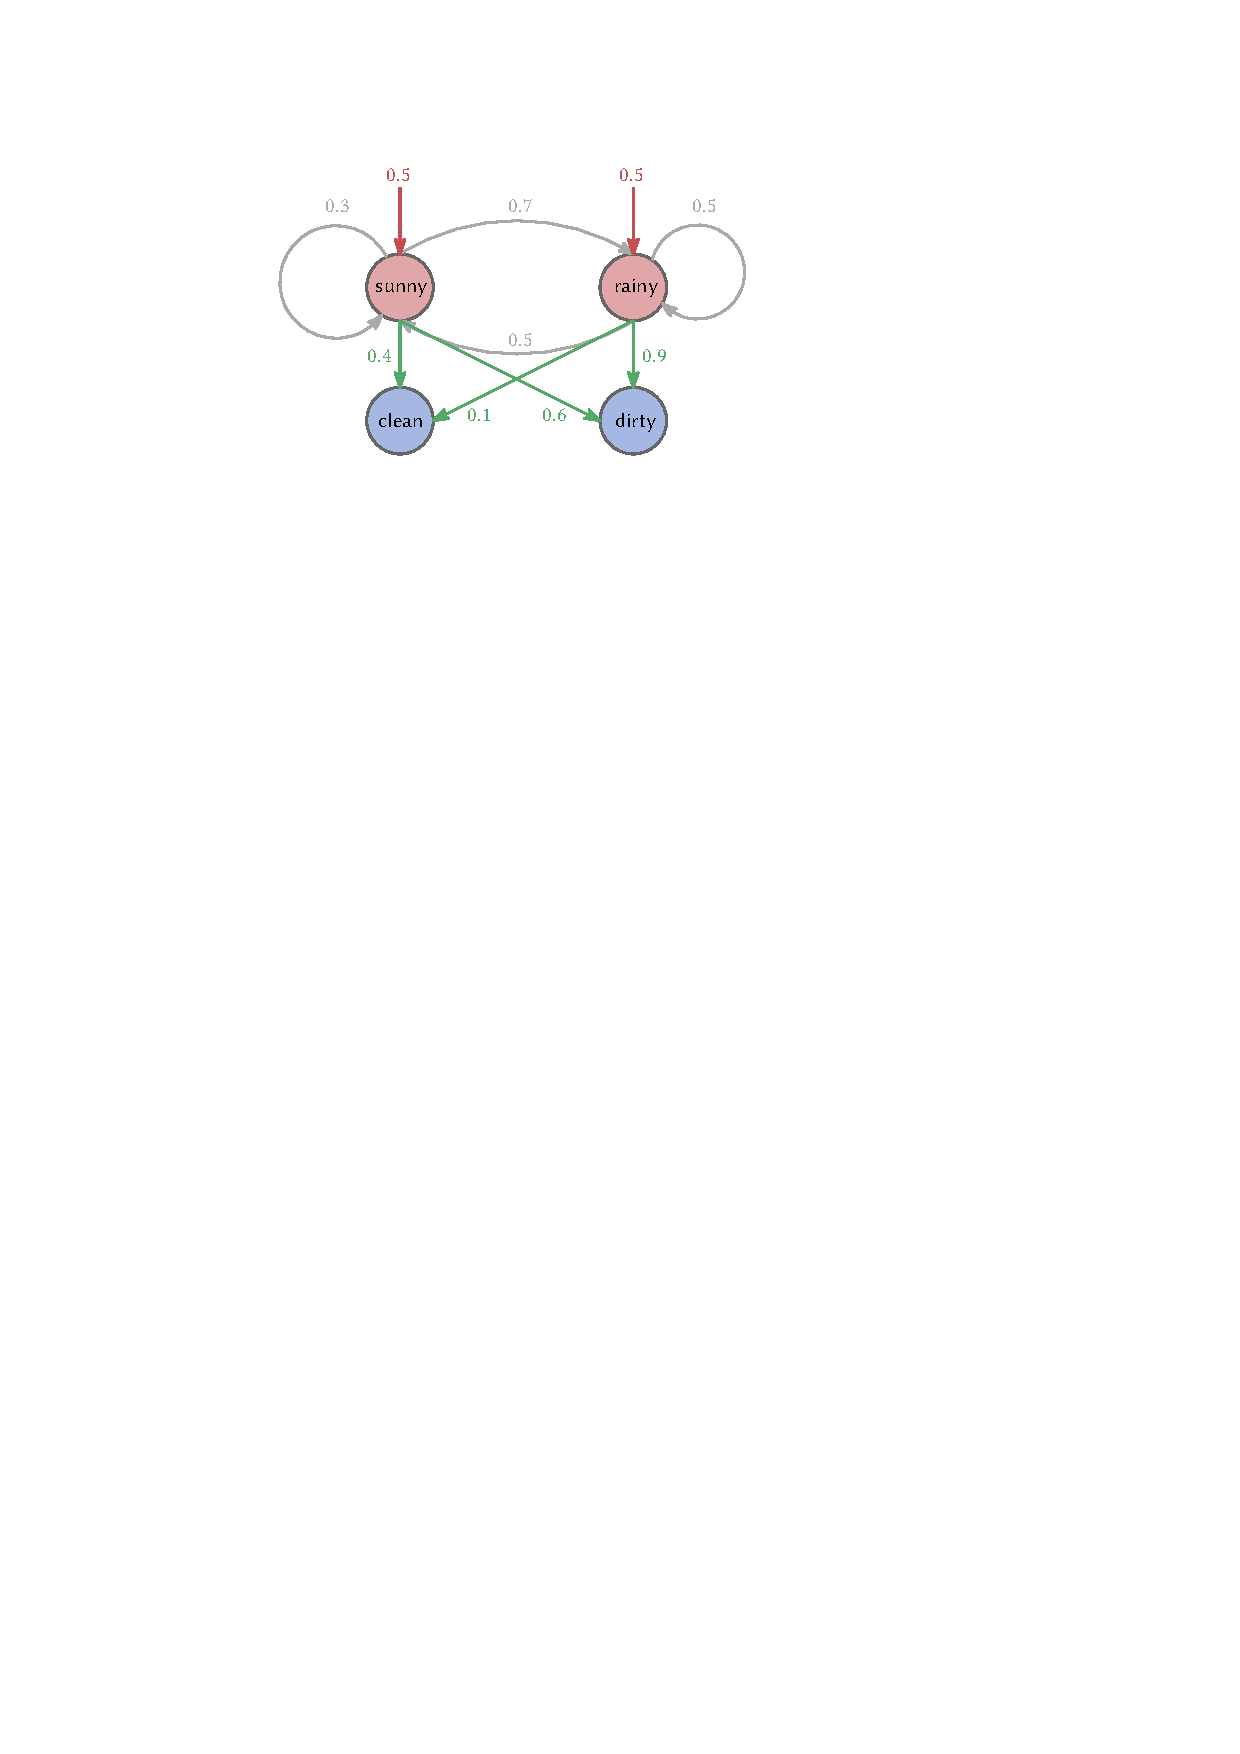
\includegraphics[width=\textwidth]{hmm-example-prison}
			\caption{Einfaches Hidden Markov Model.}
		\end{figure}
	\end{column}
\end{columns}
\end{frame}
	
\begin{frame}
	\frametitle{Einleitung}
	\framesubtitle{Datengetriebene Techniken}
	\begin{columns}
		\begin{column}{0.6\textwidth}
		\begin{block}{Datengetriebene Techniken}
			\begin{enumerate}[label=$\bullet$]
				\item \textbf{Markov-Chain (MC)}
				\item Hidden Markov Model (HMM)
				\item Neuronale Netzwerke:
				\begin{enumerate}[label=$\circ$]
					\item \textbf{Feedforward Neuronal Networks (FNN)}
					\item \textbf{Recurrent Neuronal Networks (RNN)}
					\item Transformer
					\item $\ldots$
				\end{enumerate}
				\item $\ldots$
			\end{enumerate}
			\end{block}
		\end{column}
		
		\begin{column}{0.4\textwidth}
			\begin{figure}
				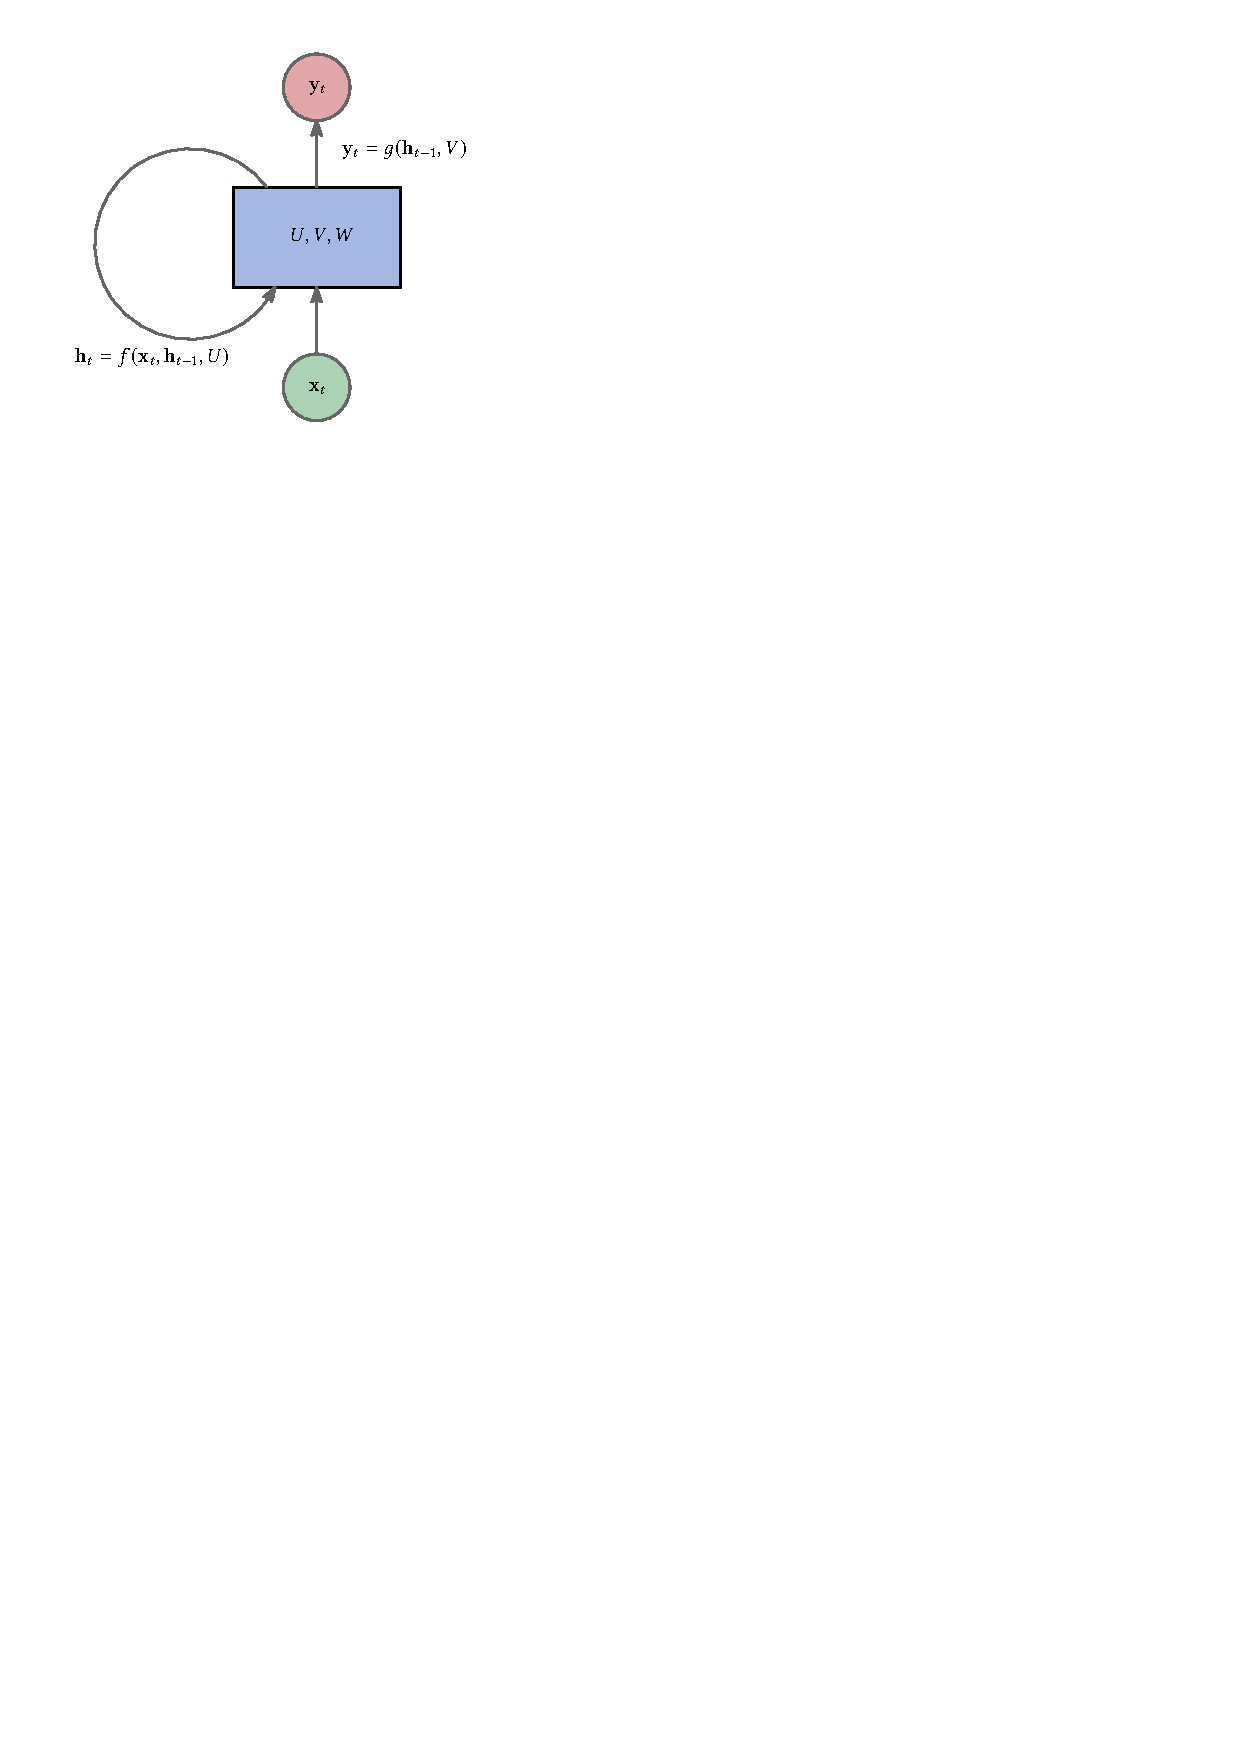
\includegraphics[width=0.9\textwidth]{rnn-diagram}
				\caption{Skizze eines RNN.}
				\label{fig:rnn-diagram}
			\end{figure}
		\end{column}
	\end{columns}
\end{frame}
	
\begin{frame}
	\frametitle{Einleitung}
	\framesubtitle{Geschichte}
	\textit{Regelbasierte} Kompositionen:
	
	\begin{enumerate}[label=$\bullet$]
		\item Guido von Arezzo (1000): Generierung von Melodien aus Text
		\item Atanasius Kirchner (1650): Automatische Erzeugung von kontrapunktischer Komposition durch hölzerne Stöcke
		\item Würfelspiele von J. K. Kirnberger  (1757 - 1812) und anderen  wie Haydn, Mozart
		\item L. Hiller und L. Isaacson (1955): \textit{\href{https://www.youtube.com/watch?v=cuq4smO_4Js}{The Iliac Suite}}, eine vollständig computergenerierte Komposition basierend auf Markov-Ketten.
		\item Iannis Xenakis (1922 - 2001) z.B. \textit{\href{https://www.youtube.com/watch?v=SZazYFchLRI}{Metastasis}}, John Cage (1912 - 1992) z.B. \textit{\href{https://www.youtube.com/watch?v=epBkVgfoXNk}{Atlas Eclipticalis}}: Zufallsbasierte Kompositionen
	\end{enumerate}
\end{frame}

\begin{frame}
	\frametitle{Einleitung}
	\framesubtitle{Geschichte}
	\textit{Datengetriebene} Kompositionen:
	
	\begin{enumerate}[label=$\bullet$]
		\item Vanilla Recurrent Neural Network (Einstimmig), \cite{todd:1989}
		\item LSTMs für Melodie und Harmonie, \cite{eck:2002}
		\item \href{https://folkrnn.org/}{FolkRNN}, LSTM (Einstimmig), \cite{sturm:2016}
		\item \href{https://www.danieldjohnson.com/2015/08/03/composing-music-with-recurrent-neural-networks/}{LSTM mit einer interessanten Architektur (Vielstimmig)}, \cite{johnson:2017}
		%\item AttentionRNN (2016)
		\item \href{https://magenta.tensorflow.org/music-transformer}{MusicTransformer}, Komposition langer Sequenzen mit erhöhter Dynamik (Vielstimmig),  \cite{huang:2018}
		\item \href{https://sites.google.com/view/anticipation-rnn-examples/accueil}{AnticipateRNN}, bedingte Melodiegenerierung (Vielstimmig),  \cite{hadjeres:2018}
		\item \href{https://ghadjeres.github.io/piano-inpainting-application/}{Transformer, bedingte Melodiegenerierung (Vielstimmig)}, \cite{hadjeres:2021}
	\end{enumerate}
\end{frame}

\begin{frame}
	\frametitle{Einleitung}
	\framesubtitle{Geschichte}
	\begin{figure}
	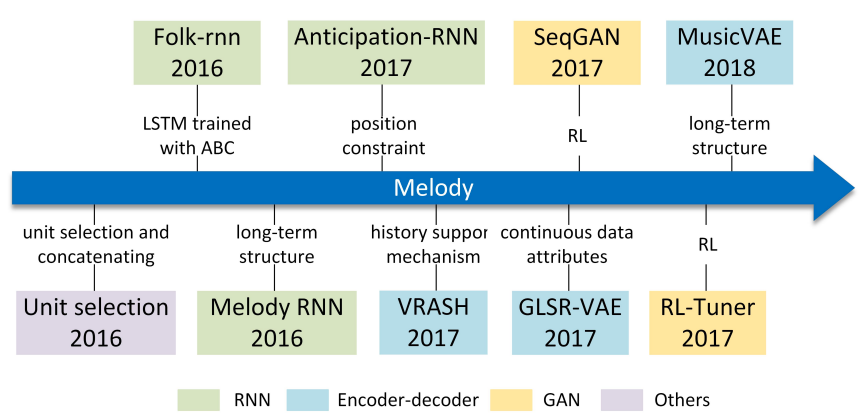
\includegraphics[width=0.9\textwidth]{melody-generation-chonology}
	\caption{Quelle: \cite{shulei:2020}}
\end{figure}
\end{frame}

\begin{frame}
	\frametitle{Einleitung}
	\framesubtitle{Geschichte}
	\begin{figure}
		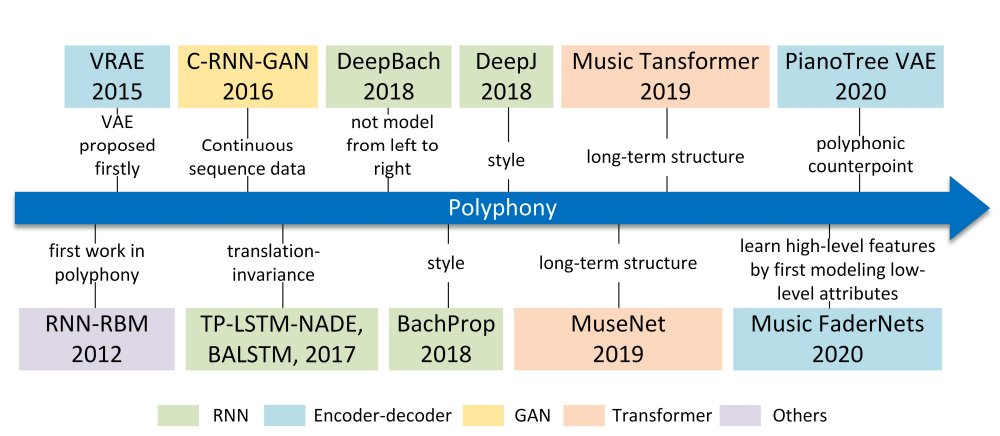
\includegraphics[width=0.9\textwidth]{polyphony-generation-chonology}
		\caption{Quelle: \cite{shulei:2020}}
	\end{figure}
\end{frame}

\begin{frame}
	\frametitle{Einleitung}
	\framesubtitle{Anwendungen}
	\begin{figure}
		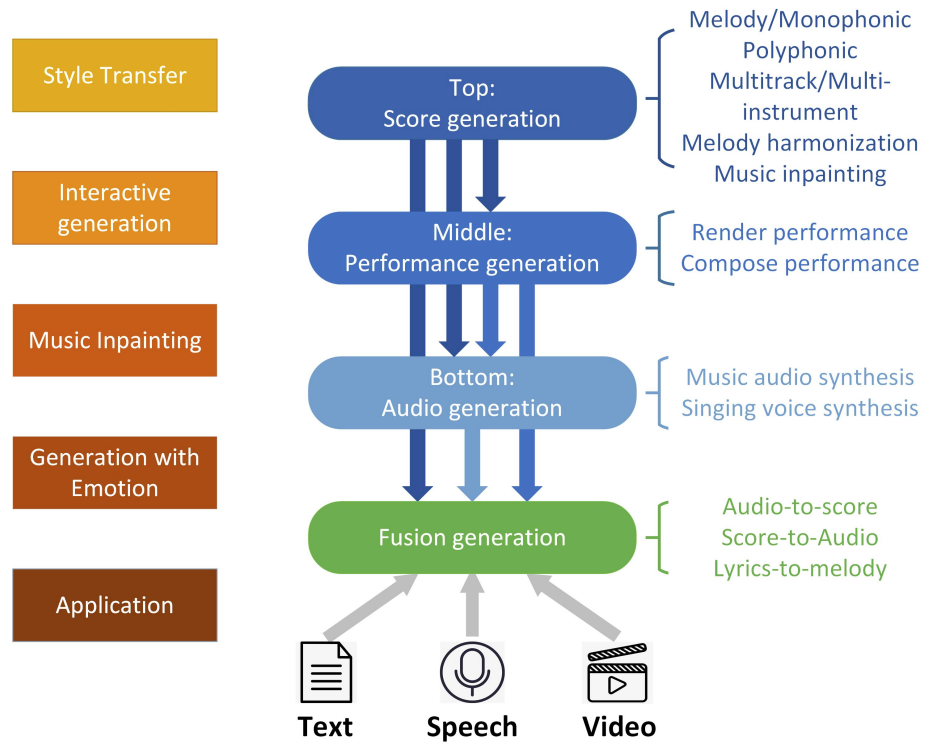
\includegraphics[width=0.54\textwidth]{possibilities}
		\caption{Quelle: \cite{shulei:2020}}
	\end{figure}
\end{frame}

\begin{frame}
	\begin{block}{Abgrenzung}
		Wir beschäftigen uns mit der \textit{abstrakten} Melodiegenerierung (ohne Harmonie).
	\end{block}
\end{frame}

\section{Repräsentationen}

\begin{frame}
	\frametitle{Repräsentationen}
	\begin{figure}
		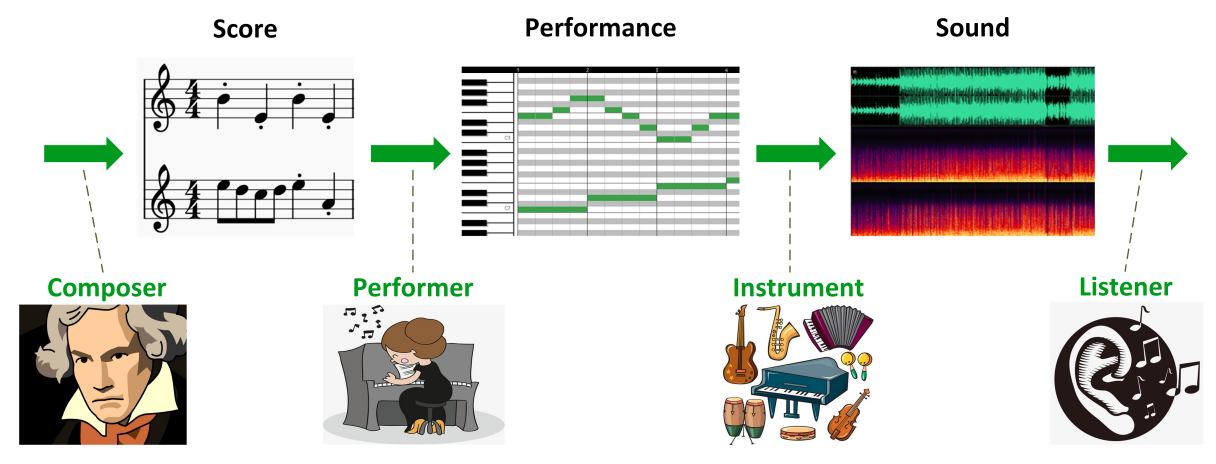
\includegraphics[width=\textwidth]{overview}
		\caption{Quelle: \cite{shulei:2020}}
	\end{figure}
\end{frame}

\begin{frame}
	\frametitle{Repräsentationen}
	Wir arbeiten mit zwei Repräsentationen:
	
	\begin{block}{(MIDI-)Notensequenz}
		Jedes Ereignis ist eine Note der Form: [Tonhöhe in MIDI]/[Dauer in Vielfache von Zeitschritt].
		Zum Beispiel entspricht 60/3 einem C3 der Länge 3/8 (Beats), wenn ein Zeitschritt 1/8 Beat wäre.
		Eine Melodie sieht dann wie folgt aus:
		\begin{center}
			64/4 55/1 53/2 $\ldots$
		\end{center}
	\end{block}
	
	\begin{figure}
		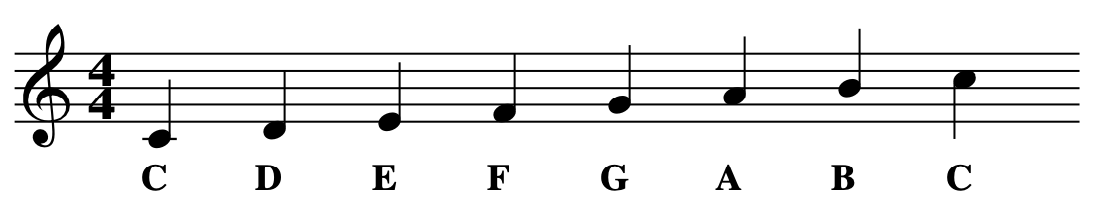
\includegraphics[width=\textwidth]{note-notation}
	\end{figure}
\end{frame}


\begin{frame}
	\frametitle{Repräsentationen}
	
	\begin{block}{Piano Roll}
		Jedes Ereignis nimmt die gleiche Zeit in Anspruch. Es gibt für jede Note ein ``Note wurde geschlagen''.
		Zudem gibt es ein Ereignis ``Note/Pause wird gehalten'' und ein Ereignis ``Pause''.
		Eine Melodie sieht dann wie folgt aus:
		\begin{center}
			64 \_ \_ \_ 55 53 \_ $\ldots$
		\end{center}
	\end{block}
	
	\begin{figure}
		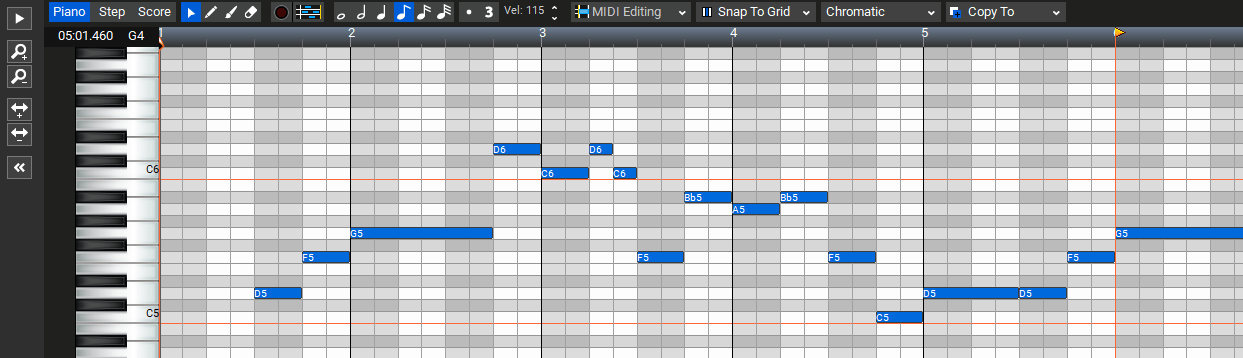
\includegraphics[width=0.8\textwidth]{piano-roll-notation}
	\end{figure}
\end{frame}

\begin{frame}
	\frametitle{Repräsentationen}
	Die \textbf{Notensequenz} benötigt ein größeres Alphabet. \textbf{Piano Roll} verwendet dafür mehr Symbole für die gleiche Information.\\
	\vspace{1cm}
	Im Falle der Vielstimmigkeit explodiert unser Alphabet!\\
	\vspace{1cm}
	\begin{block}{Frage:}
		Wie könnte unsere Repräsentation im Falle der Vielstimmigkeit aussehen?
	\end{block}
\end{frame}

\section{(Datengetriebene) Markov-Ketten}

\begin{frame}
	\frametitle{Markov-Ketten}
	\begin{block}{Problem}
		Gegeben sei eine Sequenz von Noten der Länge $n \geq 0$, generiere ``wohlkingende'' Fortsetzung.
	\end{block}
	\begin{figure}
		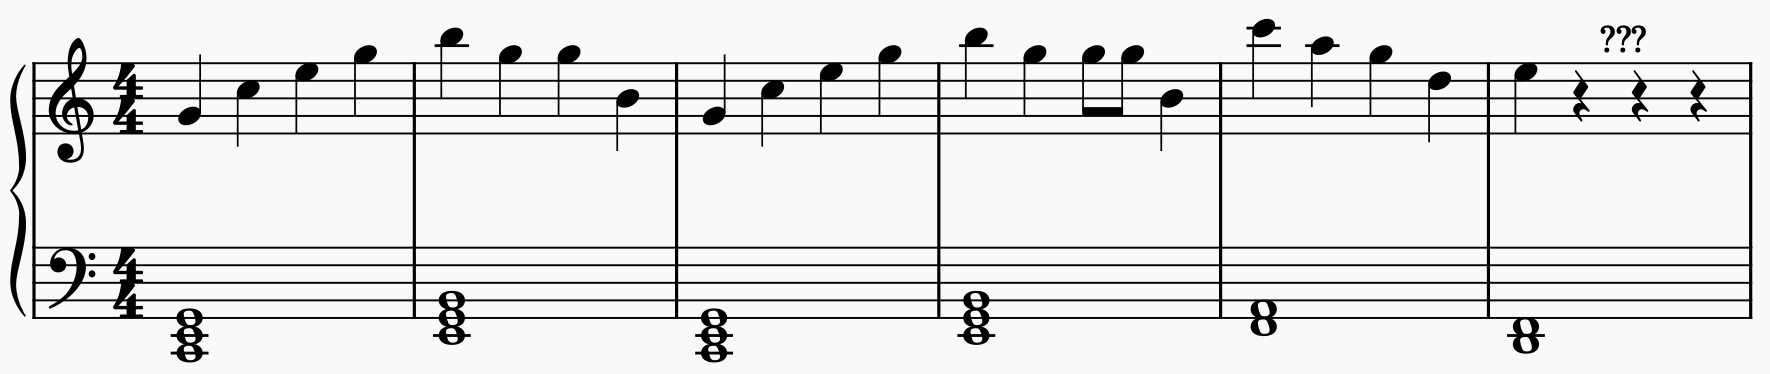
\includegraphics[width=\textwidth]{notes}
	\end{figure}
\end{frame}


\begin{frame}
	\frametitle{Markov-Ketten}
	\begin{block}{Lösungsidee}
		Fasse jede Note als Zustand eines Automaten auf und berechne die \textbf{Übergangswahrscheinlichkeiten} anhand der gegebenen Daten.
	\end{block}
		\begin{figure}
		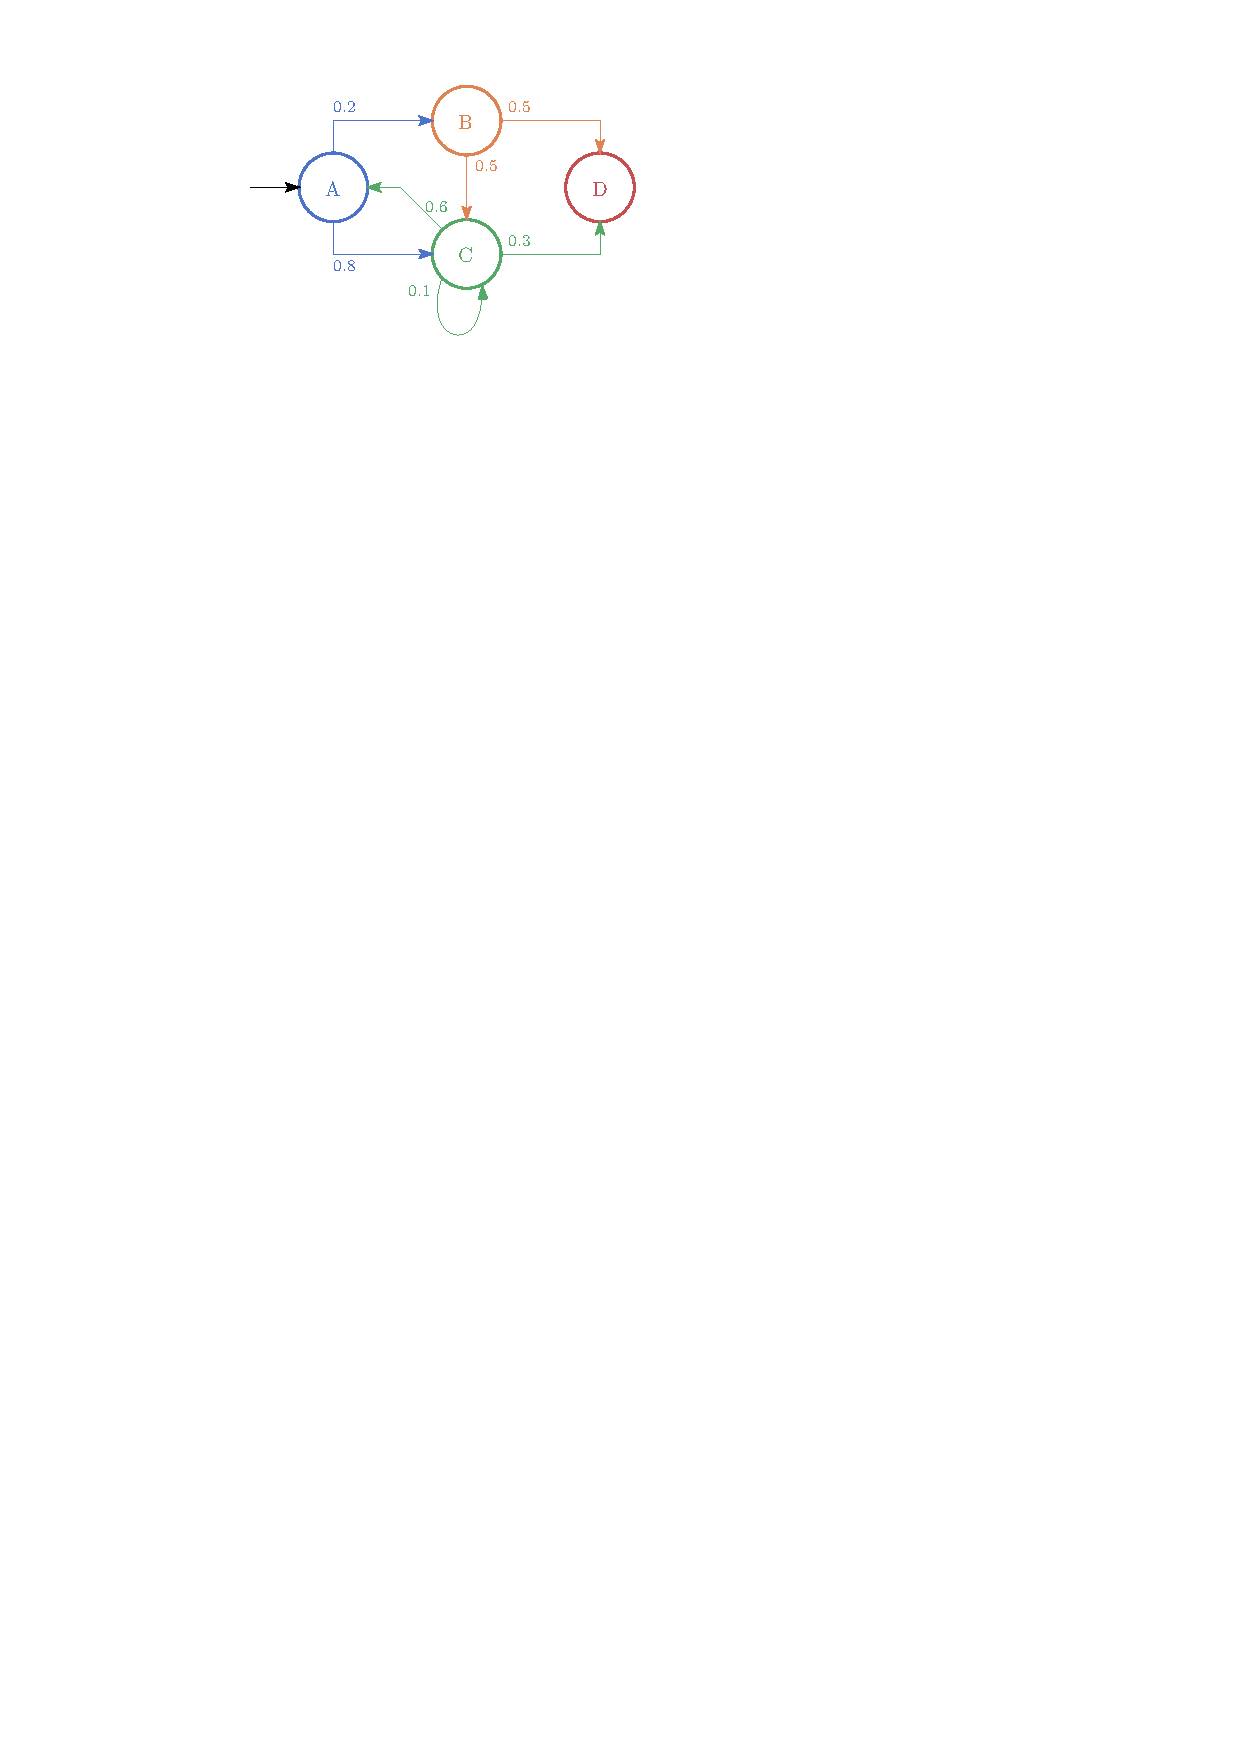
\includegraphics[width=0.4\textwidth]{markov-chain}
	\end{figure}
	Für eine solche Markov-Kette erster Ordnung hängt der nächste Zustand ausschließlich vom vorherigen ab!
\end{frame}


\begin{frame}
	\frametitle{Markov-Ketten}
	Angenommen wir haben $m$ verschiedene Noten, dann  gibt es $m^2$ Übergänge (manche haben möglicherweise eine Wahrscheinlichkeit von 0).\\
	\vspace{1cm}
	Wir gehen über alle Daten und zählen wie oft welcher Übergang auftritt.
	Anschließend teilen wir das Ergebnis durch die Anzahl der gesamten Übergänge.\\
	\vspace{1cm}
	Wir erzeugen demnach eine Tabelle oder Matrix $\mathbf{P}$ deren Zeile $j$, die Wahrscheinlichkeitsverteilung für eine die Note $j$ angibt. 
	
	$$\mathbf{p}_j = (0.6, 0.0, 0.1, 0.3)$$
	
	Eintrag $i$ in Zeile $j$ gibt demnach die Wahrscheinlichkeit für den Übergang der Note $j$ nach $i$ an.
\end{frame}


\begin{frame}
	\frametitle{Markov-Ketten}
	\begin{columns}
		\begin{column}{0.6\textwidth}
			\begin{figure}
				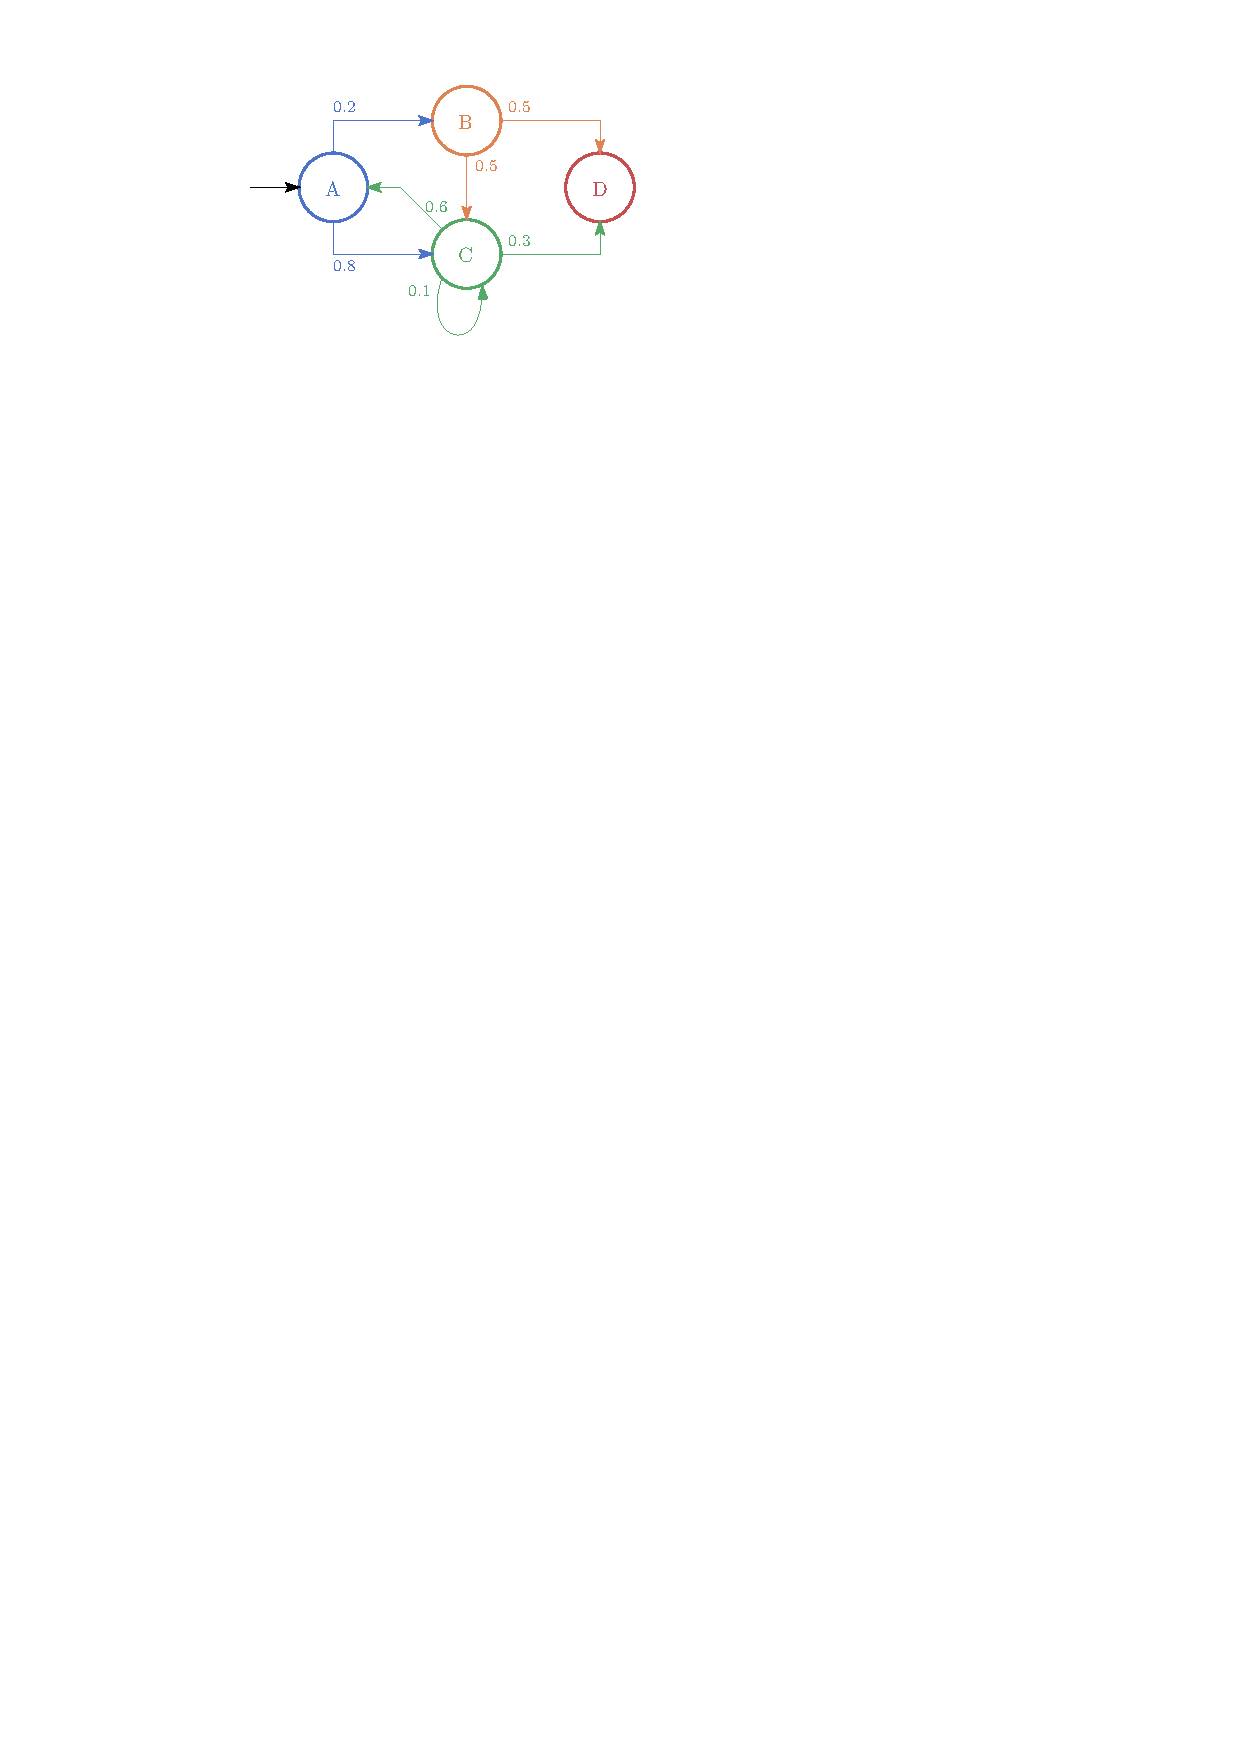
\includegraphics[width=\textwidth]{markov-chain}
			\end{figure}
		\end{column}
			\begin{column}{0.4\textwidth}
			\begin{tabular}{c | c c c c}
				 & \text{A} & \text{B} & \text{C} & \text{D} \\\hline
				\text{A} & 0.0 & 0.2 & 0.8 & 0.0 \\
				\text{B} & 0.0 & 0.0 & 0.5 & 0.5 \\
				\text{C} & 0.6 & 0.0 & 0.1 & 0.3 \\
				\text{D} & 0.0 & 0.0 & 0.0 & 0.0
			\end{tabular}
			\begin{equation*}
				\mathbf{P} = \begin{pmatrix}
					0.0 & 0.2 & 0.8 & 0.0 \\
					0.0 & 0.0 & 0.5 & 0.5 \\
					0.6 & 0.0 & 0.1 & 0.3 \\
					0.0 & 0.0 & 0.0 & 0.0
				\end{pmatrix}
			\end{equation*}
		\end{column}
	\end{columns}
\end{frame}


\begin{frame}
	\frametitle{Markov-Ketten}
	\framesubtitle{Praktikum}
	Angenommen wir hätten folgendes \textbf{(MIDI-)Notensequenz}
	\begin{center}
	. \ 64/4 \ 64/2 \ 50/3 \ 50/3 \ 64/4 \ 64/2 \ .
	\end{center}
	d.h., wir hätten 3 unterschiedliche Noten und ein spezielles Symbol: \textbf{50/3}, \textbf{64/2}, \textbf{64/4}, \textbf{.}\\
	Zählen wir nun die Übergänge:
	\begin{center}
	\begin{tabular}{c | c c c c c}
		& \text{50/3} & \text{62/2} & \text{64/4} & . \\\hline
		\text{50/3} &  1 & 0 & 1 & 0 \\
		\text{62/2} & 1 & 0 & 0 & 1\\
		\text{64/4} & 0 & 2 & 0 & 0 \\
		. & 0 & 0 & 1 & 0 \\
		\end{tabular}
	\end{center}
\end{frame}


\section{Feedforward Neural Networks}

\begin{frame}
	\frametitle{Feedforward Neural Networks}
	\begin{block}{Lösungsidee}
		Trainiere ein einfaches neuronales Netz, welches als Eingabe eine Sequenz mit $k$ Noten erhält und die nächste Note vorhersagen soll.
	\end{block}
	\begin{figure}
		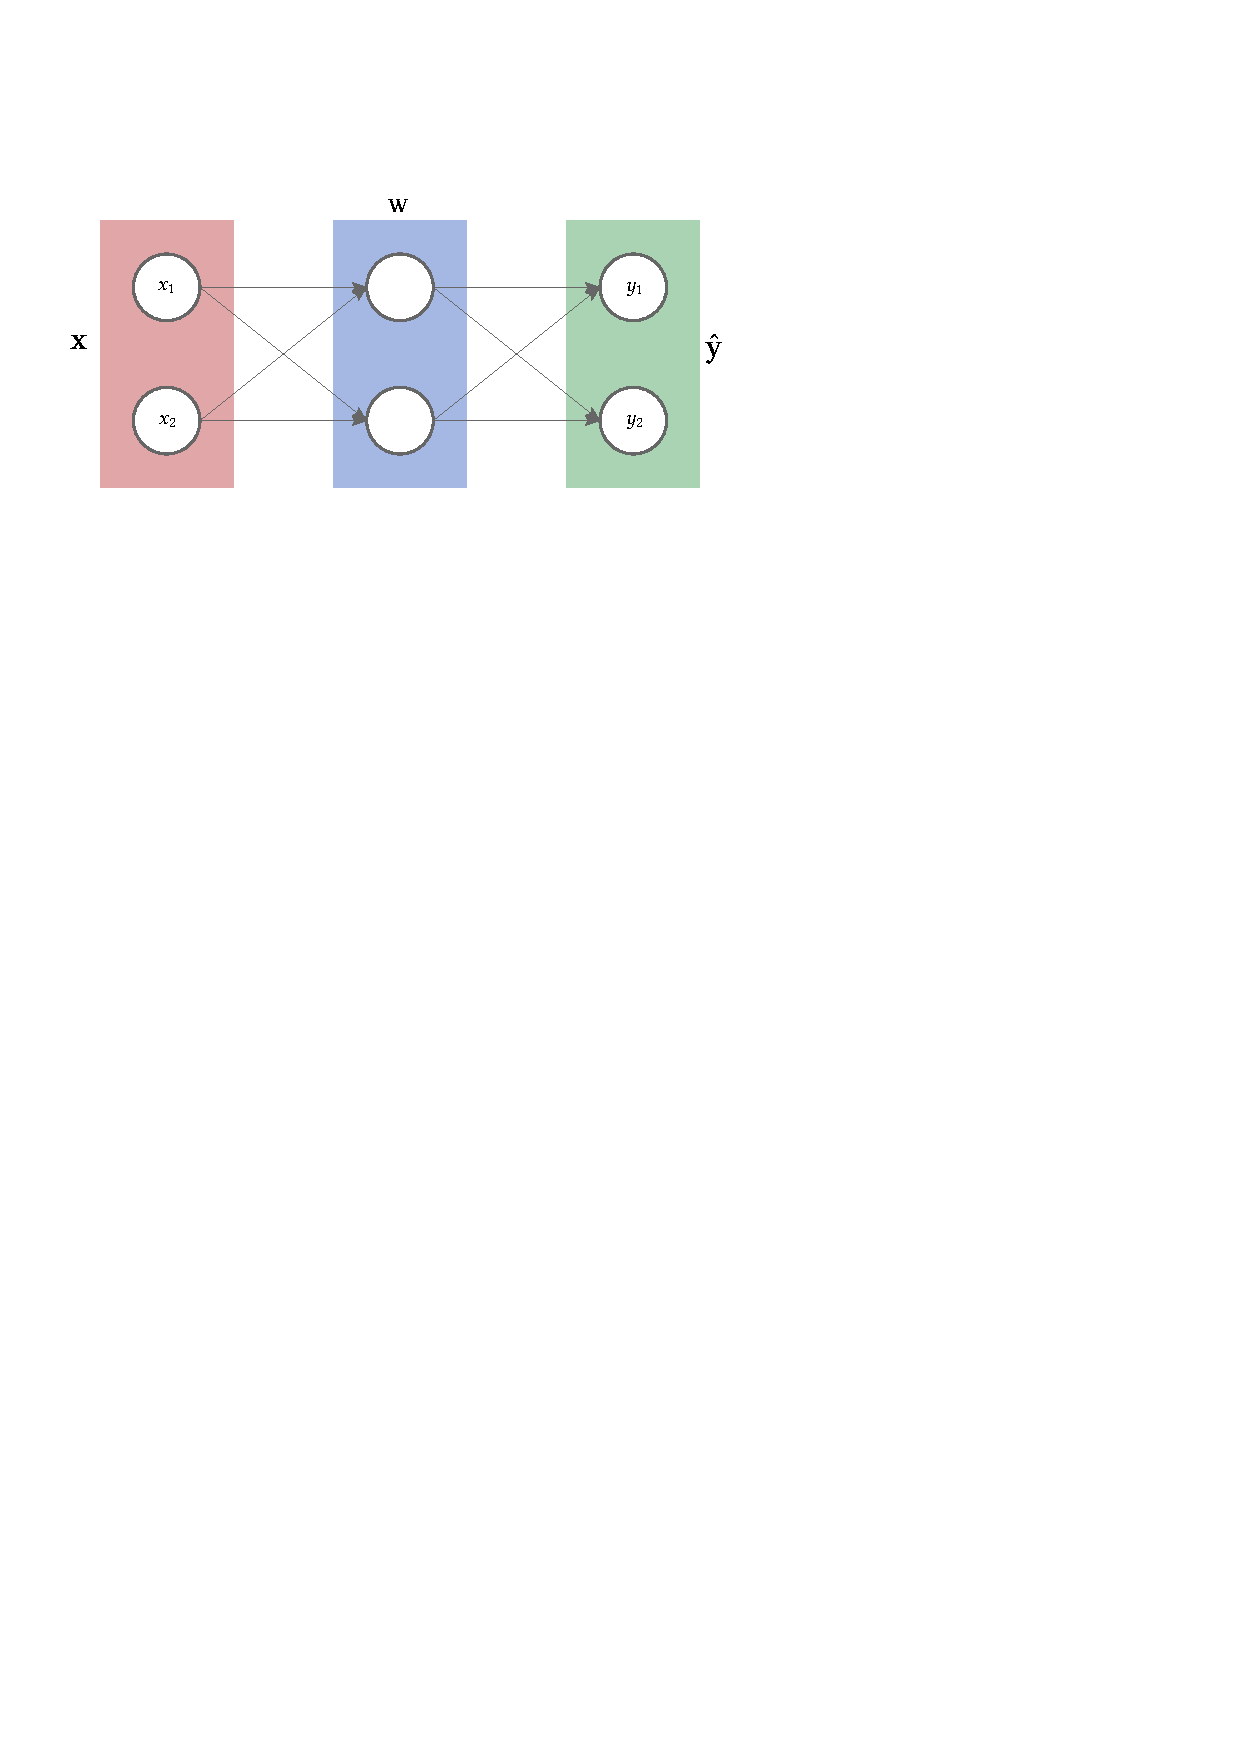
\includegraphics[width=0.5\textwidth]{fnn}
	\end{figure}
	Wir verwenden im Beispielnotebook $k=1$ und verzichten auf Aktivierungsfunktionen.
	Damit ist unser Netzwerk eine einfache $m \times m$ Matrix $\mathbf{W}$.
\end{frame}

\begin{frame}
	\frametitle{Feedforward Neural Networks}
	Jede der $m$ Noten kodieren wir mit einem sog. \textit{one-hot Vektor} mit $m$ Komponenten, wobei genau eine davon gleich 1 ist, z.B.
	
	$$\mathbf{x}^\top = (0, 0, 1, \ldots, 0, 0, 0)$$
	
	und die nächste Note $\mathbf{\hat{y}}$ ergibt sich aus
	
	$$\mathbf{x}^\top \mathbf{W} = \mathbf{\hat{y}}$$
	
	und wird als Wahrscheinlichkeitsverteilung über die $m$ Noten interpretiert.
		
\end{frame}


\begin{frame}
	\frametitle{Feedforward Neural Networks}
	\framesubtitle{Praktikum}
	Wir trainieren unser FNN mit Sequenzen der Länge $1$. D.h. aus einem Musikstück in \textbf{(MIDI-)Notensequenz}-Notation
	\begin{center}
		. \ 64/4 \ 64/2 \ 50/3 \ 50/3 \ 64/4 \ 64/2 \ .
	\end{center}
	erzeugen wir Trainingsdaten:\\
	\begin{center}
			\begin{tabular}{c c c c c c}
			. & $\Rightarrow$ & 64/4 \\
			64/4 & $\Rightarrow$ & 64/2 \\
			64/2 & $\Rightarrow$ & 50/3 \\
			50/3 & $\Rightarrow$ & 50/3 \\
			50/3 & $\Rightarrow$ & 64/4 \\
			64/4 & $\Rightarrow$ & 64/2 \\
			64/2 & $\Rightarrow$ & .
		\end{tabular}
	\end{center}
\end{frame}

\section{Recurrent Neural Networks}

\begin{frame}
	\frametitle{Recurrent Neural Networks}
	\begin{block}{Problem}
	 	In beiden Ansätzen hängt die nächste Note lediglich von der aktuellen Note ab!
	\end{block}
	\vspace{1cm}
	\begin{block}{Mögliche Verbesserungen}
		\begin{enumerate}[label=$\bullet$]
			\item Markov-Ketten höherer Ordnung
			\item Transformer (vgl. erste Woche) aka ``Lasse Netzwerk lange Sequenzen als Ganzes betrachten''
			\item \textbf{Recurrent Neural Networks} (``Netzwerk mit Speicher'')
			\item $\dots$
		\end{enumerate}
	\end{block}
\end{frame}

\begin{frame}
	\frametitle{Recurrent Neural Networks}
	\begin{figure}
		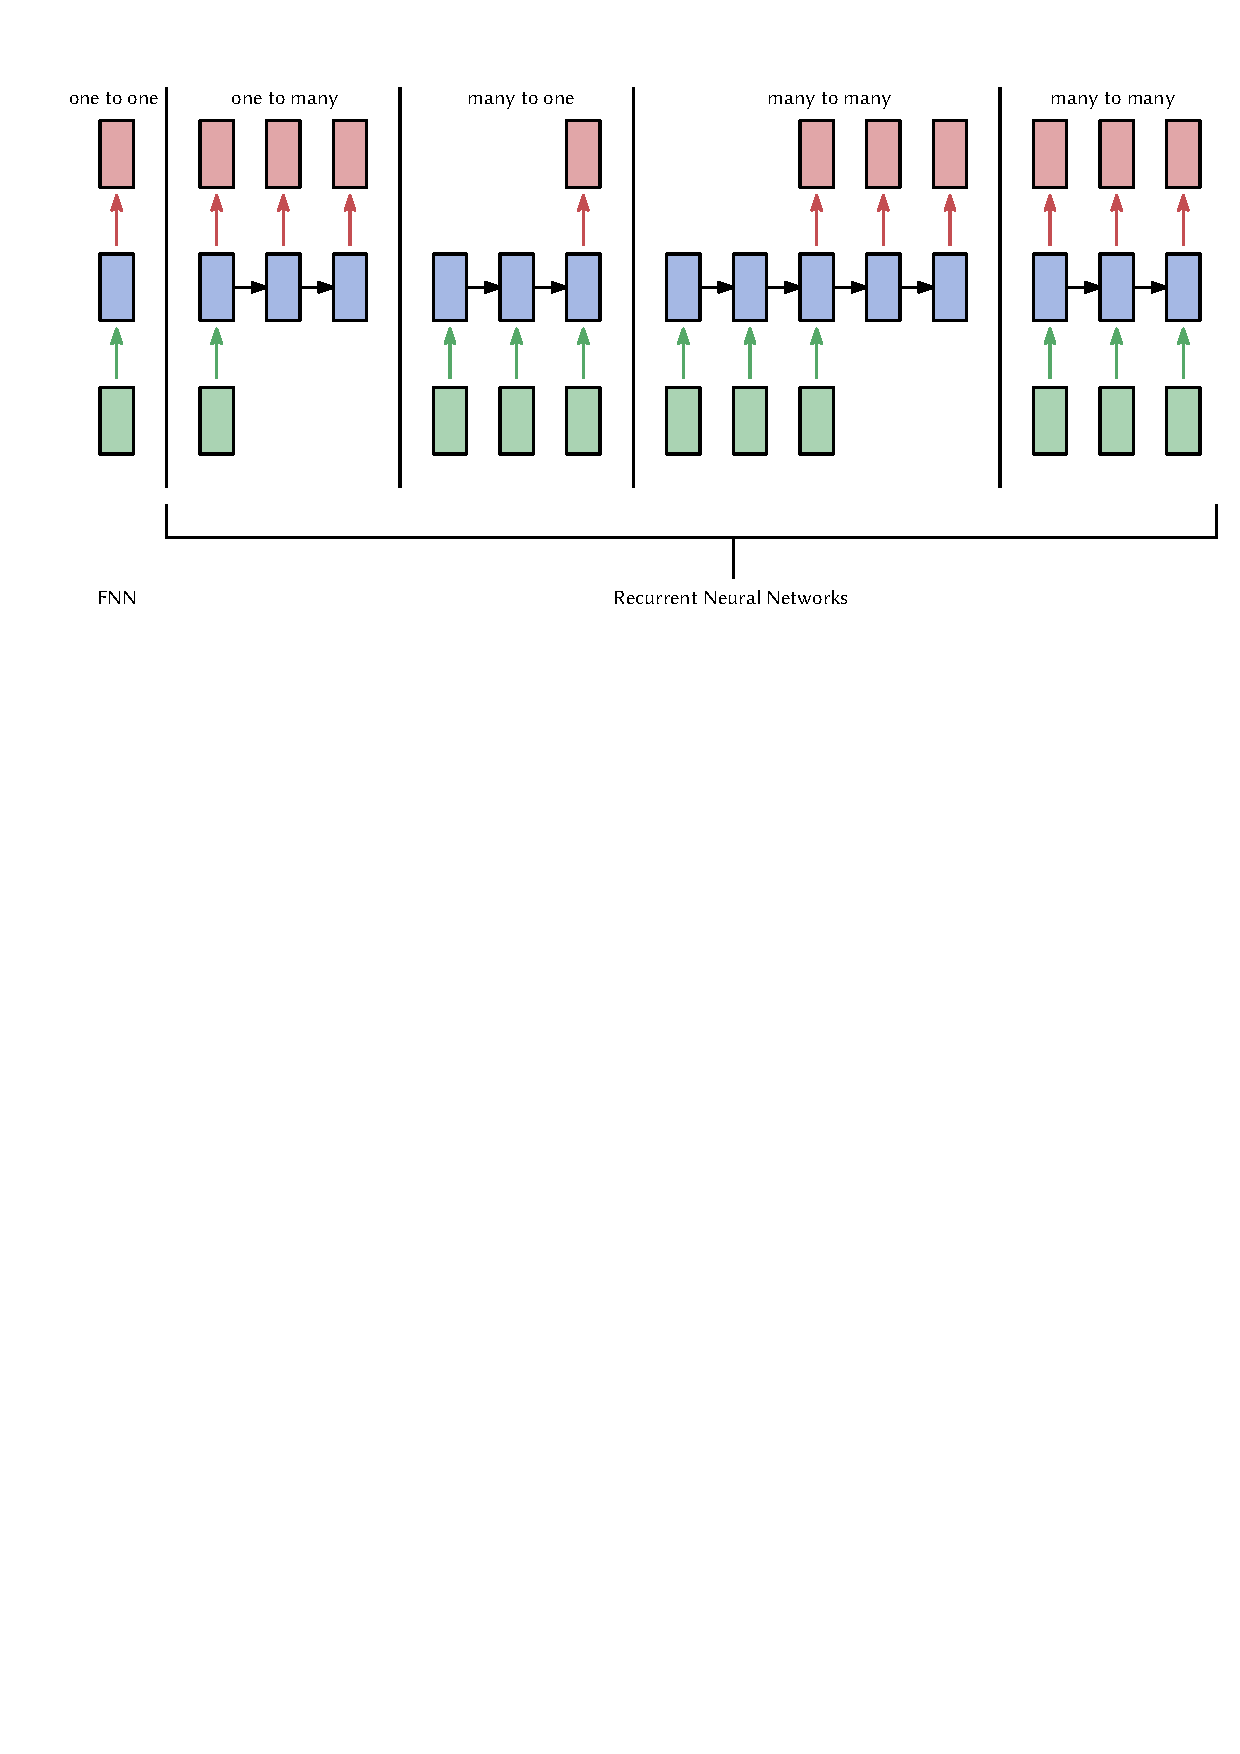
\includegraphics[width=\textwidth]{FNN-vs-RNN}
	\end{figure}
\end{frame}

\begin{frame}
	\frametitle{Recurrent Neural Networks}
	\begin{figure}
		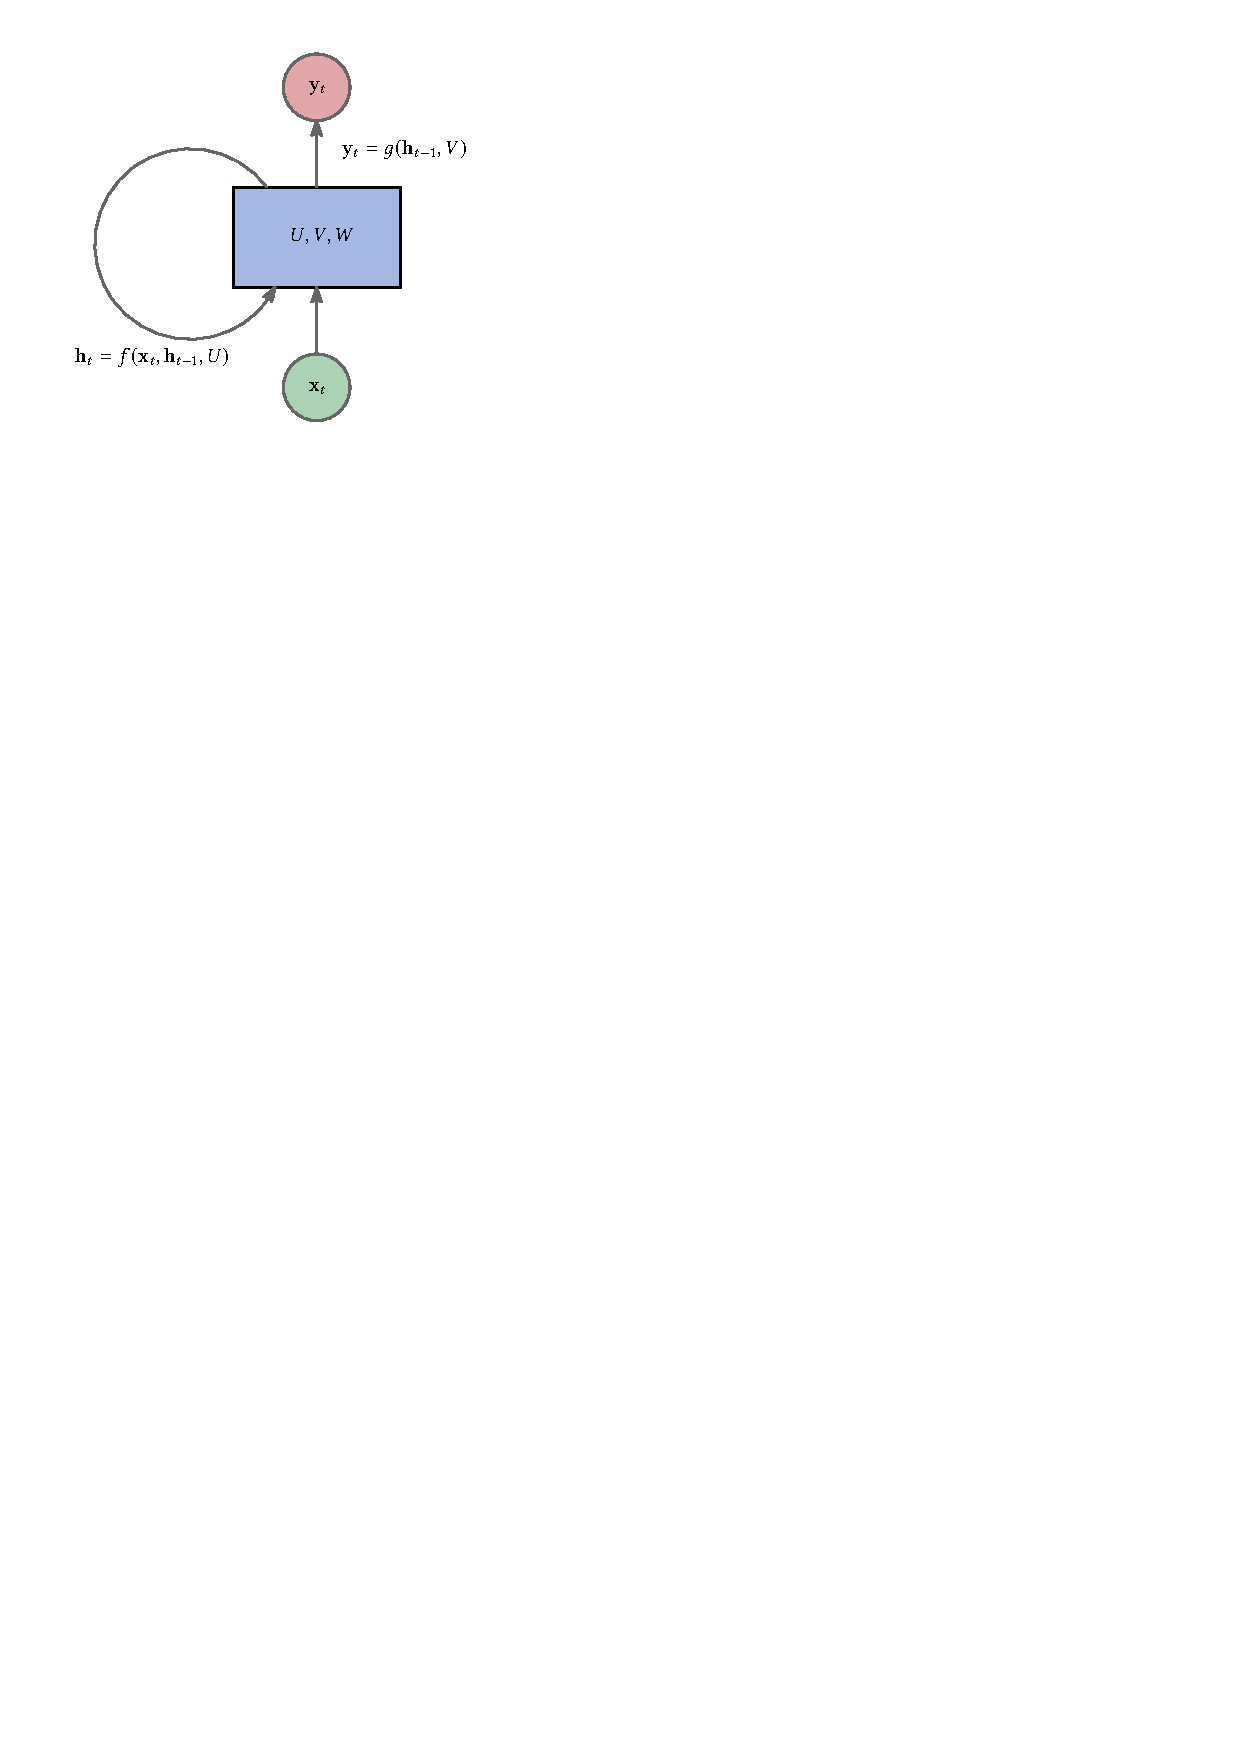
\includegraphics[scale=0.9]{rnn-diagram.pdf}
	\end{figure}
\end{frame}

\begin{frame}
	\frametitle{Recurrent Neural Networks}
	\begin{figure}
		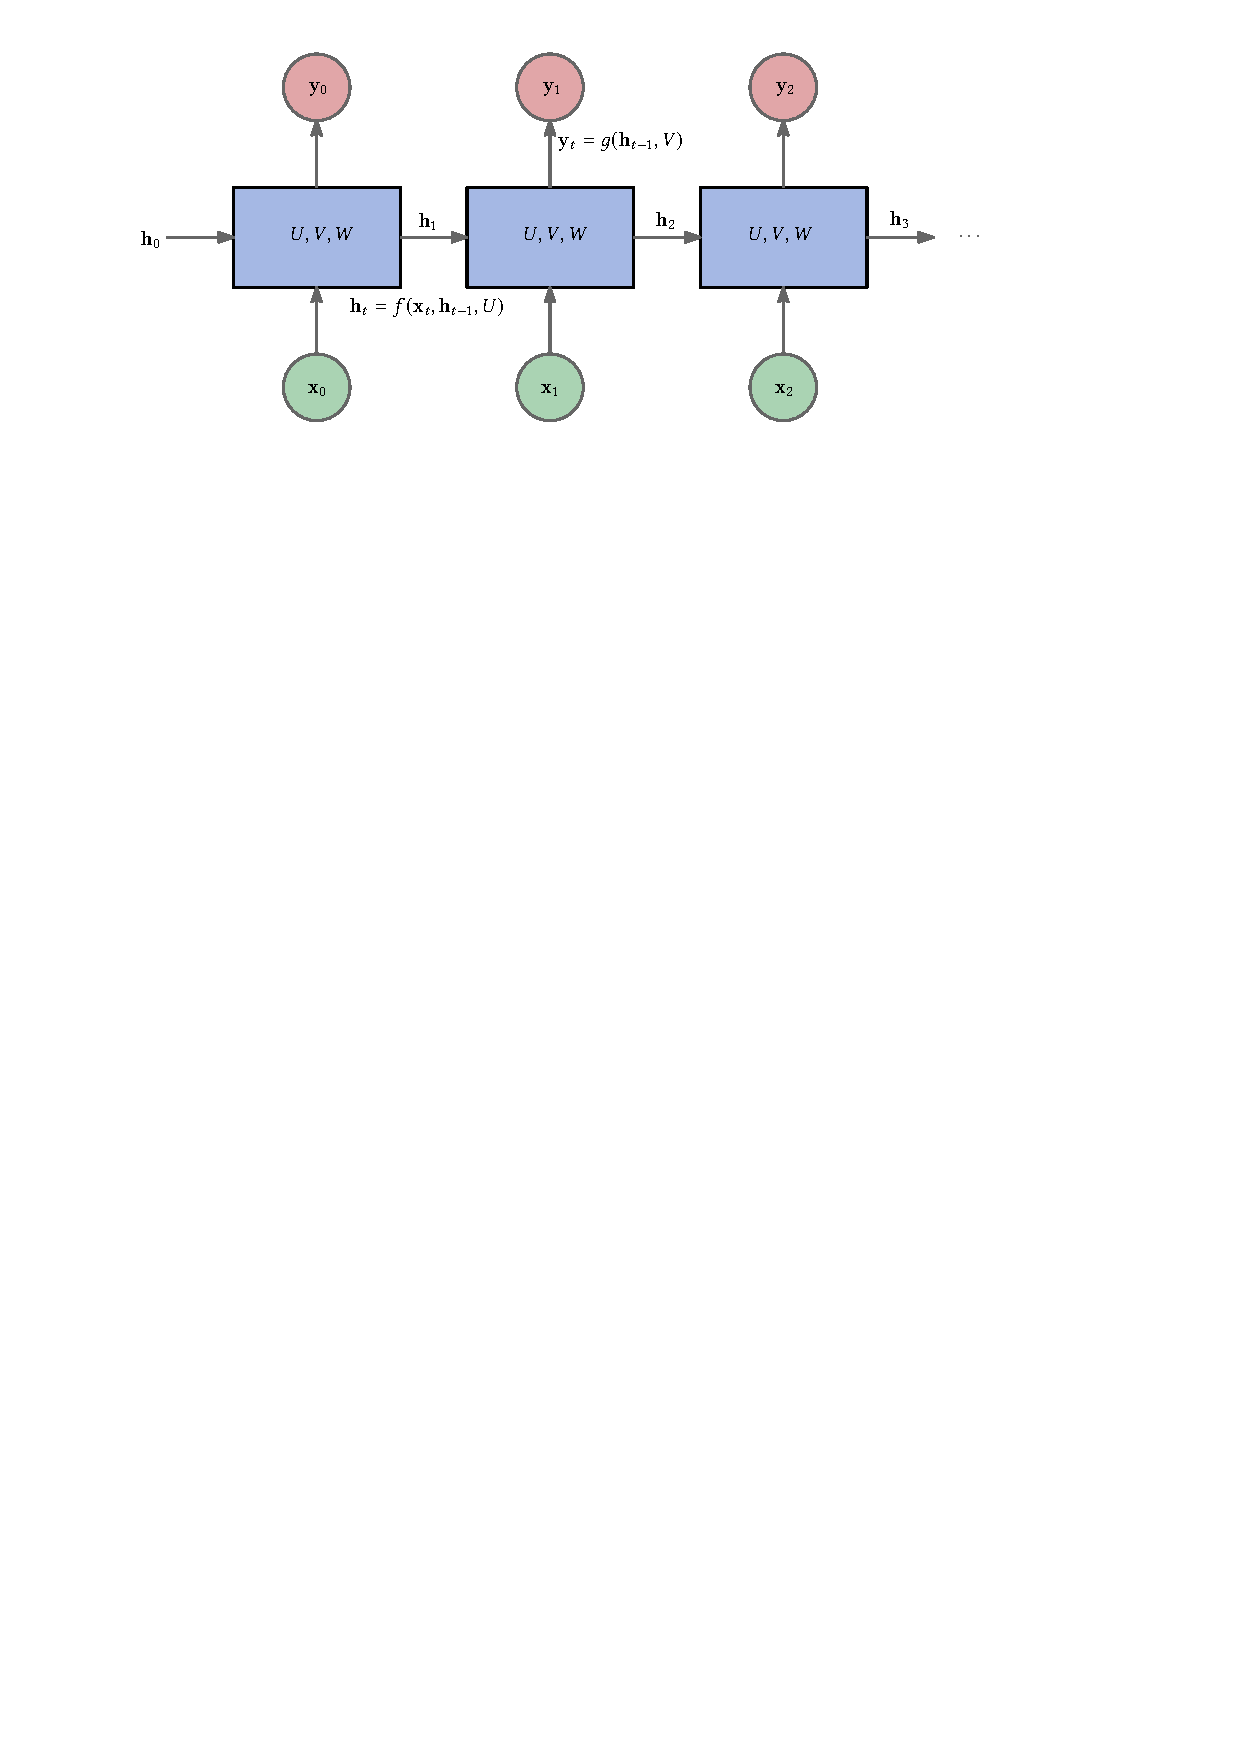
\includegraphics[scale=0.9]{rnn-diagram-unfold}
	\end{figure}
\end{frame}

\begin{frame}
	\frametitle{Recurrent Neural Networks}
	\begin{theorem}
		Für jedes \textbf{RNN} gibt es ein \textbf{Feedforward Network} mit dem gleichen Verhalten über eine endliche Zeit \cite{Rumelhart1987}.
	\end{theorem}
\end{frame}

\begin{frame}
	\frametitle{Recurrent Neural Networks}
	\framesubtitle{Back-Propagation Through Time (BPTT)}
	\begin{figure}
		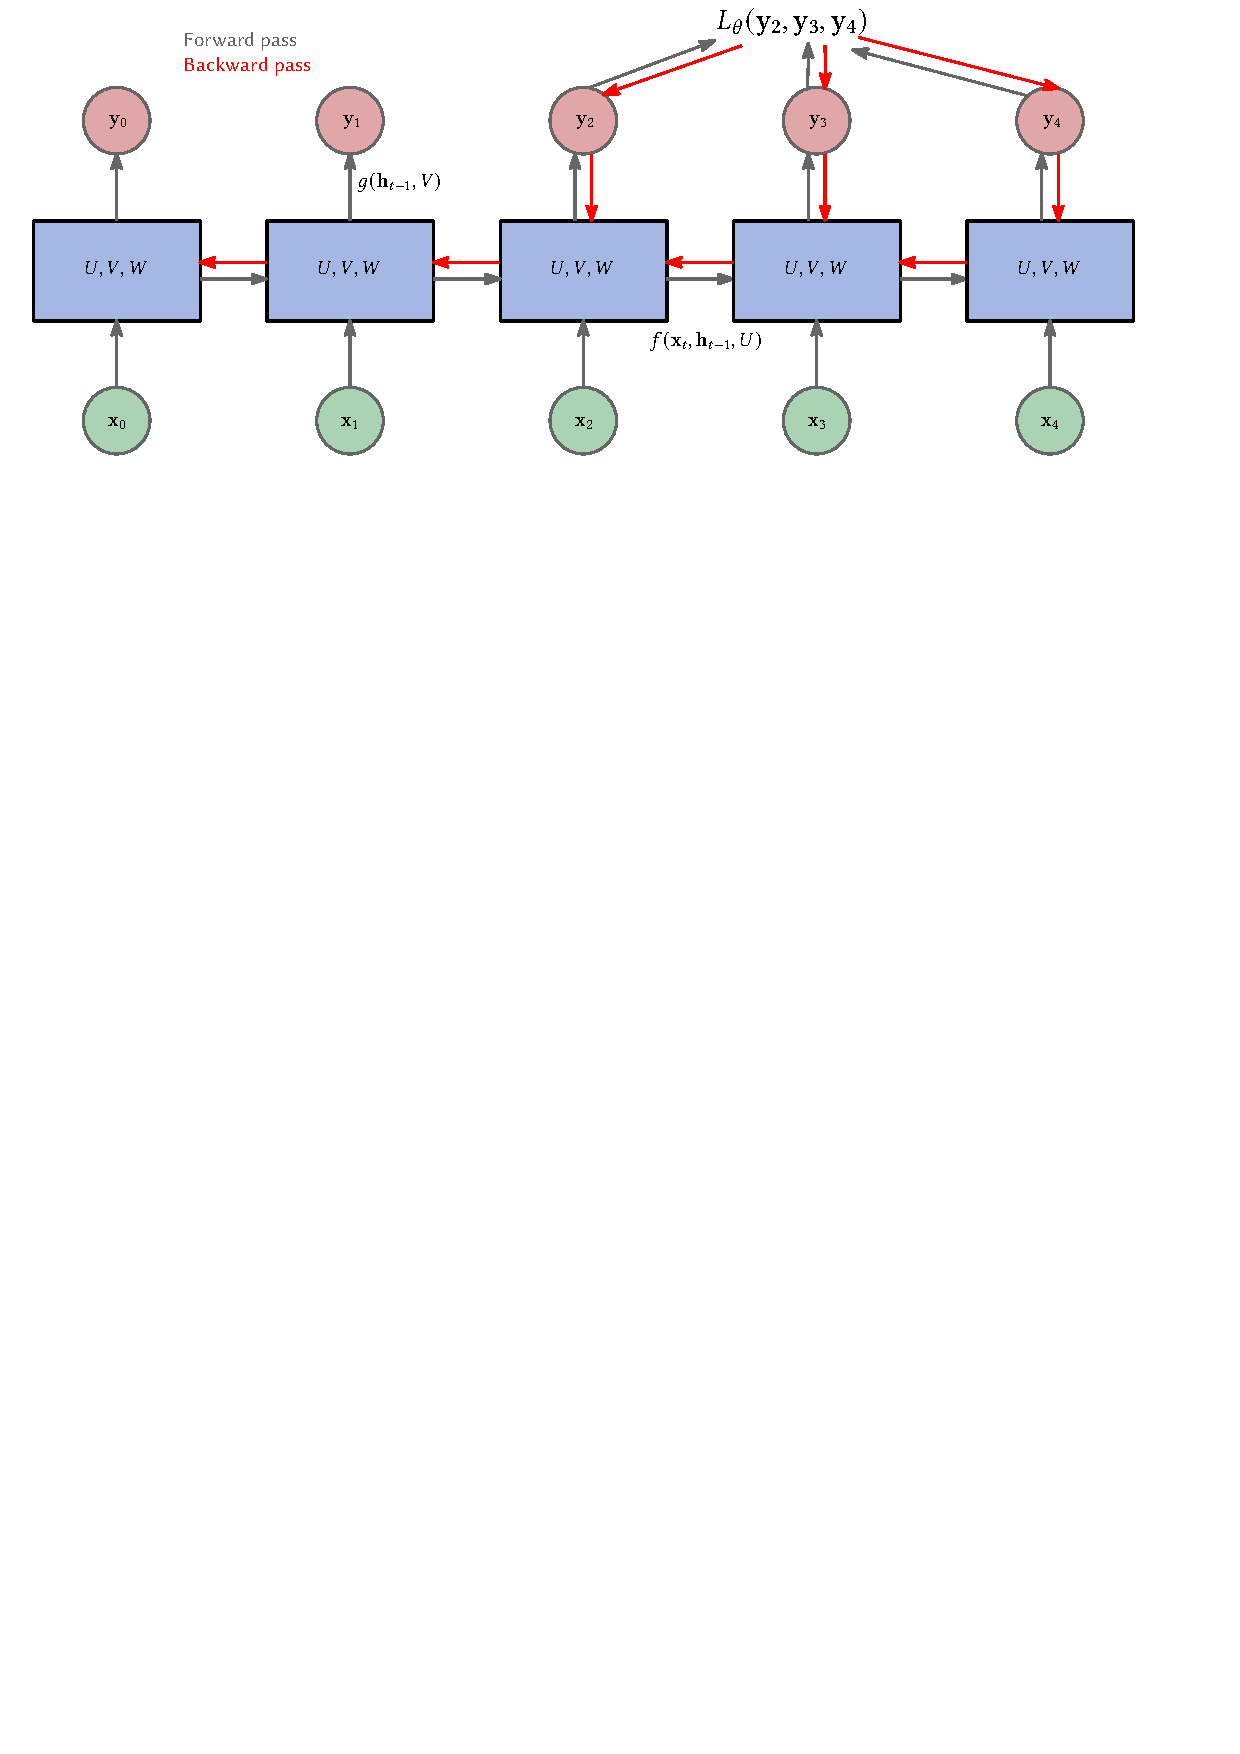
\includegraphics[width=1.0\textwidth]{bbtt}
	\end{figure}
\end{frame}

\begin{frame}
	\frametitle{Recurrent Neural Networks}
	\framesubtitle{Back-Propagation Through Time (BPTT)}
	\begin{quoting}
		``If training vanilla neural nets is optimization over functions, training recurrent nets is optimization over programs.'' -- Andrej Karpathy
	\end{quoting}
\end{frame}

\begin{frame}
	\frametitle{Recurrent Neural Networks}
	\framesubtitle{Back-Propagation Through Time (BPTT)}
	Es besteht eine exponentielle Abhängigkeit zwischen Fehler und Gewichten $W$
	\begin{equation*}
		{\color{myred}\frac{\partial \mathbf{h}_t}{\partial W}} = \frac{\partial f(\mathbf{x}_t, \mathbf{h}_{t-1}, W)}{\partial W} +  \frac{\partial f(\mathbf{x}_t, \mathbf{h}_{t-1}, W)}{\partial \mathbf{h}_{t-1}} \cdot {\color{myred}\frac{\partial \mathbf{h}_{t-1}}{\partial W}}
	\end{equation*}
	\textbf{$\Rightarrow$ Gradienten tendieren zu explodieren oder zu verschwinden.}
	\begin{equation*}
		\lim\limits_{N \rightarrow \infty}(x \cdot w_{ij}^N) = 
		\begin{cases}
			\infty & \text{ für } w_{ij} > 1.0 \\
			0 & \text{ für } w_{ij} < 1.0
		\end{cases} 
	\end{equation*}
\end{frame}

\begin{frame}
	\frametitle{Recurrent Neural Networks }
	Vanilla RNNs (in ihrer ursprünglichen Form) werden kaum noch benutzt. Stattdessen setzt man auf \textbf{Long Short-term Memory RNNs} kurz \textbf{LSTMs}.
\end{frame}

\begin{frame}
	\frametitle{Recurrent Neural Networks}
	%\framesubtitle{Probleme}
	\begin{columns}[t]
		\begin{column}{0.5\textwidth}
			\begin{block}{Vorteile}
			\begin{enumerate}[label={\color{mygreen}\textbf{+}}]
				\item Variable Eingabegröße
				\item Modellgröße explodiert nicht bei längerer Eingabe
				\item Berechnung nimmt historische Informationen auf
				\item Gewichte werden über die Zeit geteilt
			\end{enumerate}
			\end{block}
		\end{column}
		\hfill
		\begin{column}{0.5\textwidth}
			\begin{block}{Nachteile}
			\begin{enumerate}[label={\color{myred}\textbf{-}}]
				\item Langsame (sequenzielle) Berechnung
				\item Informationen die lange zurück liegen gehen verloren
				\item Keine Möglichkeit zukünftige Eingabe in die derzeitige Berechnung einzubinden
			\end{enumerate}
		\end{block}
		\end{column}
	\end{columns}
\end{frame}

\begin{frame}
	\frametitle{Recurrent Neural Networks}
	\framesubtitle{Long Short-term Memory}
	%framesubtitle{Lang- und Kurzzeitgedächtnis}
	
	\begin{figure}
		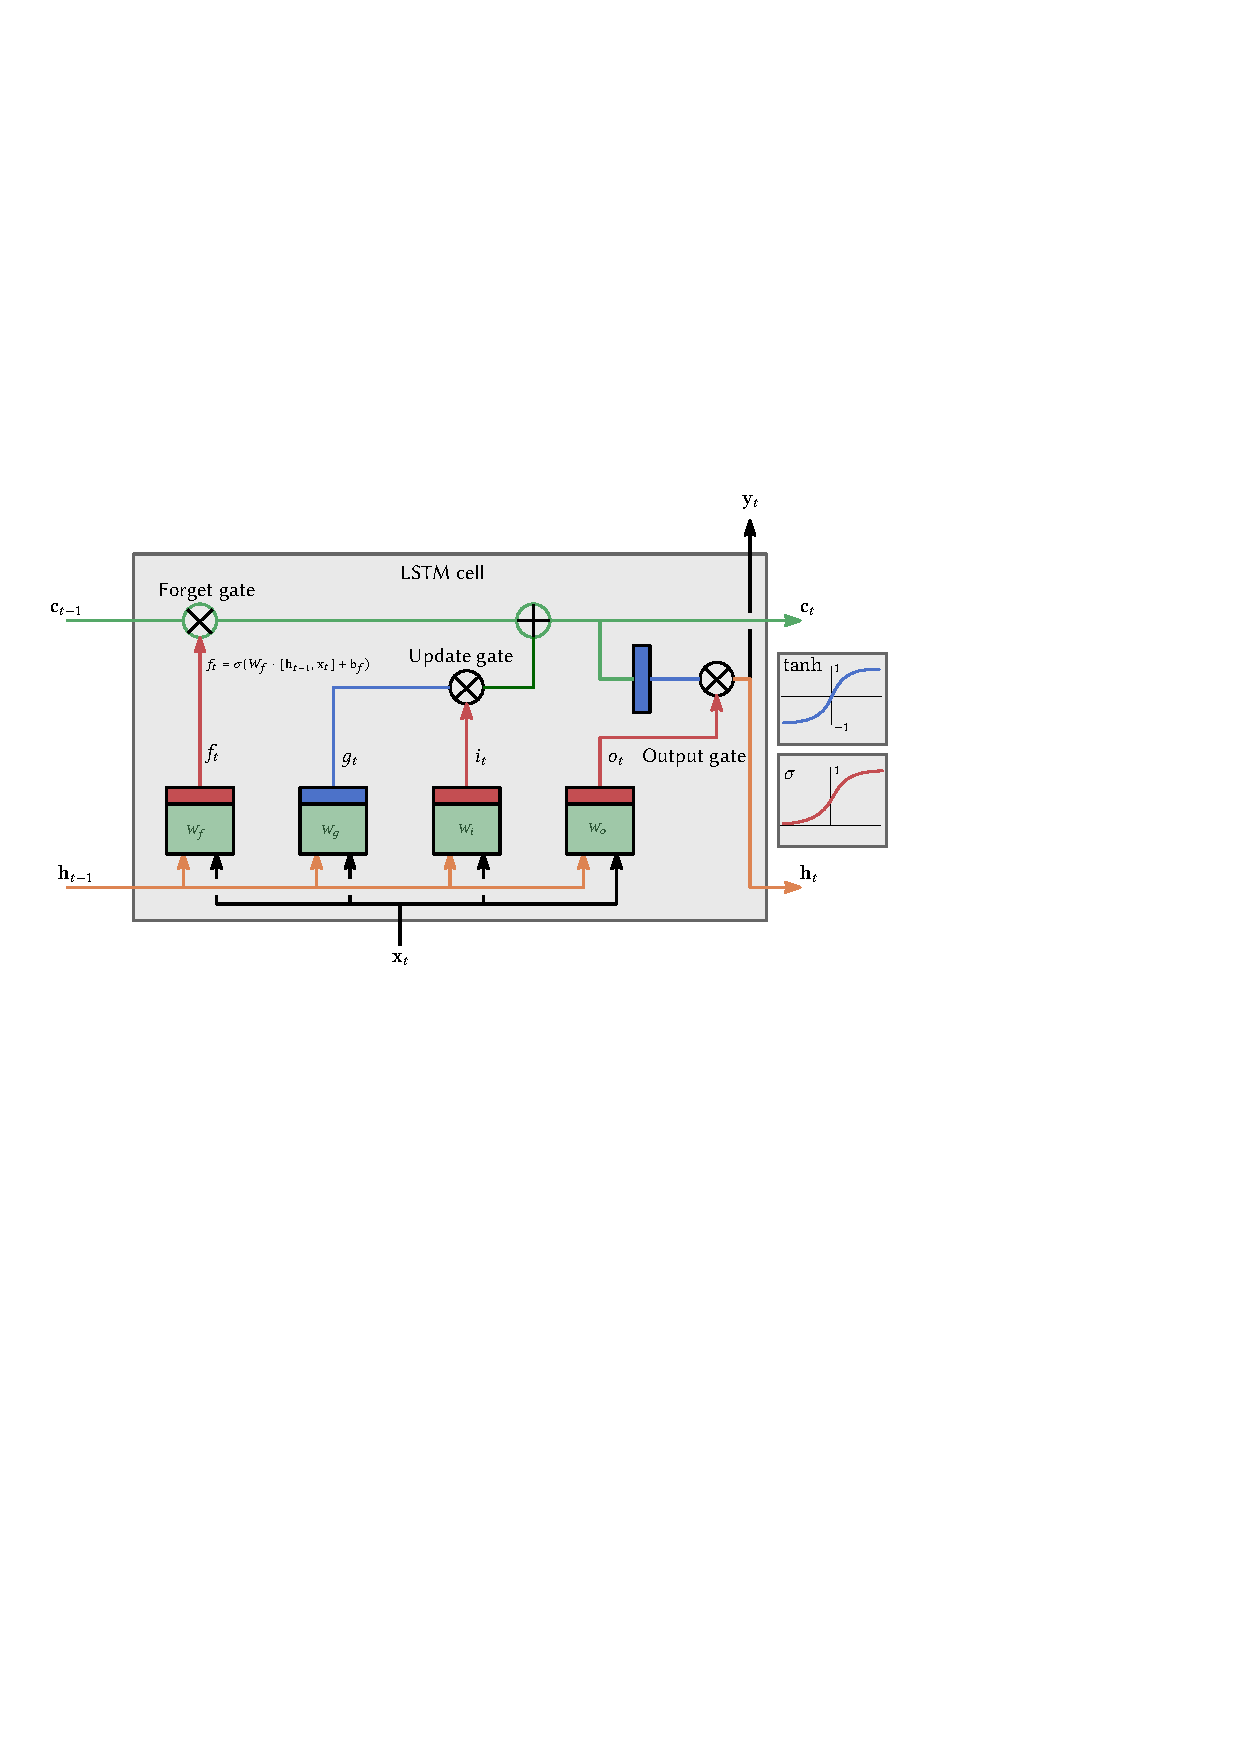
\includegraphics[width=0.9\textwidth]{lstm-cell}
	\end{figure}
	
\end{frame}

\begin{frame}
	\frametitle{Recurrent Neural Networks}
	\framesubtitle{Long Short-term Memory}
	%\framesubtitle{Probleme}
	\begin{columns}[t]
		\begin{column}{0.5\textwidth}
			\begin{block}{Vorteile (gegenüber Vanilla RNN)}
			\begin{enumerate}[label={\color{mygreen}\textbf{+}}]
				\item Kommt mit längeren Abhängigkeiten klar
				\item Stabilerer ``Speicher''
				\item Additiver statt Multiplikativer Fehler beim BPTT
			\end{enumerate}
			\end{block}
		\end{column}
		\hfill
		\begin{column}{0.5\textwidth}
			\begin{block}{Nachteile (gegenüber Vanilla RNN)}
			\begin{enumerate}[label={\color{myred}\textbf{-}}]
				\item Längeres Training mit mehr Ressourcen
				\item Anfällig für Überanpassung
				%	\item Keine Möglichkeit zukünftige Eingabe in die derzeitige Berechnung einzubinden
				%	\item Gradientenproblem nicht vollständig gelöst
			\end{enumerate}
			\end{block}
		\end{column}
	\end{columns}
	\vspace{1.0cm}
	Die sequenzielle Struktur, d.h. der \textbf{Informationsfluss durch die Zeit} bleibt bestehen!\\
	\vspace{0.5cm}
	$\Rightarrow$ Die Information wird weiterhin mit der Zeit verwischt.
\end{frame}

\begin{frame}
	\frametitle{Recurrent Neural Networks}
	\framesubtitle{Praktikum}
	Nehmen wir an, wir trainieren unser RNN mit Sequenzen der Länge $4$. D.h. aus einem Musikstück in \textbf{Piano Roll}-Notation
	\begin{center}
		64 \_ \_ \_ 55 53 \_ 63 \_ \_ \_ r \_ \_ \_ 55 \_ \_ \_ 56 \_ \_ \_ 
	\end{center}
	erzeugen wir Trainingsdaten:\\
	\begin{center}
	\begin{columns}[t]
		\begin{column}{0.4\textwidth}
			\begin{tabular}{c c c c c c}
				. & . & . & . & $\Rightarrow$ & 64 \\
				. & . & . & 65 & $\Rightarrow$ & \_ \\
				. & . & 65 & \_ & $\Rightarrow$ & \_ \\
				. & 65 & \_ & \_ & $\Rightarrow$ & \_ \\
				65 &  \_ & \_ & \_ & $\Rightarrow$ & 55 \\
				\_ & \_ & \_ & 55 & $\Rightarrow$ & 53 \\
				& & & $\ldots$ & & 
			\end{tabular}
		\end{column}
			\begin{column}{0.4\textwidth}
			\begin{tabular}{c c c c c c}
				& & & $\ldots$ & & \\
				\_ & 56 & \_ & \_ & $\Rightarrow$ & \_  \\
				56 & \_ & \_ & \_ & $\Rightarrow$ & .  \\
				\_ & \_ & \_ & . & $\Rightarrow$ & . \\
				\_ & \_ & . & . & $\Rightarrow$ & . \\ 
				\_ & . & . & . & $\Rightarrow$ & . 
			\end{tabular}
		\end{column}
	\end{columns}
\end{center}
\end{frame}

\begin{frame}[allowframebreaks]
	\frametitle{Referenzen}
	{\scriptsize% dirty fix for the non-chapter bib
		\bibliographystyle{apalike}
		\bibliography{references.bib}}
\end{frame}

\end{document}